%**************************************************************************************************************
% A Classic Thesis Style
% An Homage to The Elements of Typographic Style
%
% Copyright (C) 2025 André Miede and Ivo Pletikosić
%
% If you like the style then I would appreciate a postcard. My address
% can be found in the file ClassicThesis.pdf. A collection of the
% postcards I received so far is available online at
% http://postcards.miede.de
%
% License:
% This program is free software; you can redistribute it and/or modify
% it under the terms of the GNU General Public License as published by
% the Free Software Foundation; either version 2 of the License, or
% (at your option) any later version.
%
% This program is distributed in the hope that it will be useful,
% but WITHOUT ANY WARRANTY; without even the implied warranty of
% MERCHANTABILITY or FITNESS FOR A PARTICULAR PURPOSE.  See the
% GNU General Public License for more details.
%
% You should have received a copy of the GNU General Public License
% along with this program; see the file COPYING.  If not, write to
% the Free Software Foundation, Inc., 59 Temple Place - Suite 330,
% Boston, MA 02111-1307, USA.
%
% PLEASE SEE ALSO THE AUTHORS' NOTE REGARDING THIS LICENSE
% IN THE DOCUMENTATION (ClassicThesis.pdf --> Chapter 1 / Chapter01.tex)
% **************************************************************************************************************
\RequirePackage{silence} % :-\
  % caused by classicthesis
  \WarningFilter{scrreprt}{Usage of package `titlesec'}
  \WarningFilter{scrreprt}{Usage of package `tocloft'}
  \WarningFilter{titlesec}{Non standard sectioning command}
  % caused by babel
  \WarningFilter{tracklang}{No `datatool' support for dialect `ngerman'}
  % caused by pdfx
  \WarningFilter{hyperref}{Option `pdftex' has already been used}
  \WarningFilter{pdfx}{Setting all color commands to rgb}

% -- TemplateKnob
\documentclass[
  % layout options (keep this)
  paper=a4,               % define the paper size
  fontsize=11pt,          % define the font size
  headinclude,            % count the header as part of the text area
  footinclude,            % count the footer as part of the text area
  % cleardoublepage=empty,  % page style used for inserted interleaf pages
  % print-first options (for duplex printing and binding; comment when using screen-first options)
  % twoside,                % use mirrored inner/outer margins
  openright,              % start parts, chapters, ... on right-hand (odd-numbered) pages
  BCOR=5mm,               % binding correction (adjust as needed)
  % screen-first options (for PDF viewing; comment when using print-first options)
  twoside=false,          % use a one-sided layout (\cleardoublepage won't insert interleaf pages)
  %openany,                % allow parts, chapters, ... to start on any page
  %BCOR=0mm,               % no binding correction required
  % content options (adjust to your liking)
  numbers=noenddot,       % numbers of sectioning commands are set without a final point
  titlepage,              % create title on a separate page
  captions=tableheading   % adjust spacing below OR above table captions (don't mix styles!):
                          % - captions above tables (recommended): set captions=tableheading
                          % - captions below tables: set captions=tablesignature
]{scrreprt}

%********************************************************************
% Note: Make all your adjustments in here
%*******************************************************
% !TeX root = Thesis.tex

% ****************************************************************************************************
% classicthesis-config.tex
% formerly known as loadpackages.sty, classicthesis-ldpkg.sty, and classicthesis-preamble.sty
% Use it at the beginning of your ClassicThesis.tex, or as a LaTeX Preamble
% in your ClassicThesis.{tex,lyx} with % !TeX root = Thesis.tex

% ****************************************************************************************************
% classicthesis-config.tex
% formerly known as loadpackages.sty, classicthesis-ldpkg.sty, and classicthesis-preamble.sty
% Use it at the beginning of your ClassicThesis.tex, or as a LaTeX Preamble
% in your ClassicThesis.{tex,lyx} with % !TeX root = Thesis.tex

% ****************************************************************************************************
% classicthesis-config.tex
% formerly known as loadpackages.sty, classicthesis-ldpkg.sty, and classicthesis-preamble.sty
% Use it at the beginning of your ClassicThesis.tex, or as a LaTeX Preamble
% in your ClassicThesis.{tex,lyx} with \input{classicthesis-config}
% ****************************************************************************************************
% If you like the classicthesis, then I would appreciate a postcard.
% My address can be found in the file ClassicThesis.pdf. A collection
% of the postcards I received so far is available online at
% http://postcards.miede.de
% ****************************************************************************************************

% set important options before any package can load any of the packages below
\PassOptionsToPackage{dvipsnames}{xcolor} % for classicthesis (e.g. pass before loading tikz)
\PassOptionsToPackage{hyperfootnotes=false,pdfa}{hyperref} % for classicthesis and pdfx

% ****************************************************************************************************
% 0. Set the encoding of your files. UTF-8 is the only sensible encoding nowadays. If you can't read
% äöüßáéçèê∂åëæƒÏ€ then change the encoding setting in your editor, not the line below. If your editor
% does not support utf8 use another editor!
% ****************************************************************************************************
\usepackage[utf8]{inputenc}
\usepackage[T1]{fontenc} % T2A for cyrillics


% ****************************************************************************************************
% 1. Configure classicthesis for your needs here, e.g., remove "drafting" below
% in order to deactivate the time-stamp on the pages
% ****************************************************************************************************
\PassOptionsToPackage{
	% -- TemplateKnob
	drafting=true,            % print version information on the bottom of the pages
	tocaligned=false,         % the left column of the toc will be aligned (no indentation)
	dottedtoc=true,           % page numbers in ToC flushed right
	eulerchapternumbers=true, % use AMS Euler for chapter font (otherwise Palatino)
	floatperchapter=false,    % numbering per chapter for all floats (i.e., Figure 1.1)
	eulermath=true,           % use awesome Euler fonts for mathematical formulae (only with pdfLaTeX)
	beramono=true,            % toggle a nice monospaced font (w/ bold)
	palatino=false,            % deactivate standard font for loading another one, see the last section at the end of this file for suggestions
	%linedheaders=true,       % obsolete / available for backwards compatibility
	style=classicthesis       % classicthesis, arsclassica, linedheaders, plain
}{classicthesis}

% classicthesis overrides for special Makefile test targets
\ifdefined\injectCToptions
	\injectCToptions
\fi

% ****************************************************************************************************
% 2. Language, time and dates, personal data and custom classicthesis template modifications
% ****************************************************************************************************
\usepackage[ngerman,american]{babel} % change this to your language(s), main language last
% Spanish languages need extra options in order to work with this template
%\usepackage[spanish,es-lcroman]{babel}
\usepackage[useregional]{datetime2} % for formatting dates (load after babel/polyglossia)
\usepackage{etoolbox}
% load personal information like title, name, dates, ...
\input{00-definitions/PersonalInfo}

\PassOptionsToPackage{
	% -- TemplateKnob (also have a look into classicthesis-seemoo.sty for further options)
	layout=standard,      % pick from standard, balanced, tight and dense (not recommended)
	% layout definitions:
	%   - standard: the default classicthesis layout with big margins (~69 CPL, 46 lines)
	%   - balanced: wider text area, but still useful margins (~75 CPL, 42 lines)
	%   - tight: even wider text area, tight margin, BCOR > 5 mm looks bad (~77 CPL, 41 lines)
	%   - dense: tiny margins, BCOR > 5 mm almost impossible, not recommended (~87 CPL, 46 lines)
	% how to pick:
	%   - I want to use margin notes --> standard or balanced (tight can be ok with BCOR <= 5 mm)
	%   - I value readability (<80 CPL, up to ~500 words per page) --> standard, balanced, tight
	%   - I have lots of plots and tables --> balanced, tight, dense
	%   - I need as much text as possible per page --> dense
	% notes:
	%   - standard, balanced and tight are roughly equal in the amount of information per page
	%   - balanced and tight are optimized for dina4 with 11 pt Palatino font
	osf=false,            % enable old style figure fonts (not recommended)
	cleantoc=false,       % remove less important chapters from the ToC
	%hidefrontbackmatter, % hide the front and back matter PDF bookmarks
	titleiscover=true,    % treat the title page as the cover (i.e. center the title page)
	%parts,               % use parts (as in a book; for long theses only!)
	%phd,                 % use for a full-blown PhD thesis (with parts, author references, etc.)
	%version=0.1.0,       % when drafting: the version number is displayed on the bottom of the pages
}{classicthesis-seemoo}

% classicthesis-seemoo overrides for special Makefile test targets
\ifdefined\injectCTSoptions
	\injectCTSoptions
\fi
% ****************************************************************************************************


% ****************************************************************************************************
% 3. Loading some handy packages
% ****************************************************************************************************

% ********************************************************************
% BibLaTeX for compiling bibliographies
% ********************************************************************
\usepackage[%
	backend=biber,bibencoding=utf8, % instead of bibtex
	sorting=snyt,                   % shorthand, name, year, title
	maxbibnames=10,                 % default: 3, et al.
	defernumbers=true,              % enable so split references (author's publications) have continuous numbers
	natbib=true,                    % natbib compatibility mode (\citep and \citet still work)
	language=auto,
	style=numeric-comp
]{biblatex}
\DeclareSortingTemplate{snyt}{
	\sort{
		\field{shorthand}
	}
	\sort{
		\field{author}
	}
	\sort{
		\field{year}
	}
	\sort{
		\field{title}
	}
}

% ********************************************************************
% General useful packages
% ********************************************************************
\usepackage[fleqn]{amsmath} % math environments and more by the AMS (fleqn=flush left equations)
\usepackage{graphicx}       % include figures (jpg, png, pdf, ...)
\usepackage{scrhack}        % fix warnings when using KOMA with listings package
\usepackage{xspace}         % to get the spacing after macros right

% optional packages for certain document variants or specific problems
\usepackage[autostyle=true]{csquotes} % for citing in the PhD statement
%\usepackage[LabelsAligned,NoDate]{currvita} % nice cv style for PhD theses (required for the CV)
\usepackage{pdfpages}                % include papers, e.g., for cumulative PhD theses
%\usepackage{xurl}                    % break URLs within word boundaries (not recommended)

% useful packages for drafting
\usepackage{lipsum}         % for generating template text
\usepackage{todonotes}      % manage todos with todonotes

% ********************************************************************
% TikZ and PGFPlots
% ********************************************************************
\usepackage{tikz}
\usepackage{pgfplots}
\pgfplotsset{compat=newest}
\usetikzlibrary{
	chains,
	positioning,
	quotes,
}

\def\StripPrefix#1>{}
\def\isOverleaf{\fi
	\def\overleafJobname{output}% overleaf defaults to 'output' as \jobname
	\edef\overleafJobname{\expandafter\StripPrefix\meaning\overleafJobname}%
	\edef\job{\jobname}%
	\ifx\job\overleafJobname
		}

		% To cache tikz pictures you have to run pdflatex with -shell-escape or --enable-write18
		\ifnum\pdfshellescape=1
			\usepgfplotslibrary{external}
			\if\isOverleaf
				\tikzexternaldisable
			\else
				\tikzexternalize
			\fi
		\fi

		% Lengths for matlab2tikz
		\newlength\figureheight
		\newlength\figurewidth
		% ****************************************************************************************************


		% ****************************************************************************************************
		% 4. Setup floats: tables, (sub)figures, and captions
		% ****************************************************************************************************
		\graphicspath{{06-pictures/}} %path for figures
		\usepackage{float}
		\usepackage{tabularx} % better tables
		\usepackage{booktabs}   % professionelle Tabellenlinien
		\usepackage{longtable}  % mehrseitige Tabellen
		\usepackage{pdflscape}  % Querformat für einzelne Seiten
		\setlength{\extrarowheight}{3pt} % increase table row height
		\usepackage{multirow} % for table cells spanning multiple rows
		\usepackage{subcaption} % for subfigures, subtables, ... (subcaption supersedes subfig)
		\usepackage{makecell}
		% ****************************************************************************************************


		% ****************************************************************************************************
		% 5. Setup code listings
		% ****************************************************************************************************
		\usepackage{listings}
		\lstset{
		% color scheme follows template
		commentstyle=\color{CTsemi},
		keywordstyle={\color{CTtitle}},
		stringstyle=\color{CTcitation},
		basicstyle=\ttfamily\lst@ifdisplaystyle\small\fi, % use normal font size in \lstinline
	emphstyle={\color{CTlink}},
	tabsize=2,
	showstringspaces=false,
	captionpos=b, % caption below listing
	breaklines=true,
	frame=tb,
	numberstyle=\scriptsize,
	numbers=left,
	stepnumber=1,
	numbersep=8pt,
}
% ****************************************************************************************************


% ****************************************************************************************************
% 6. Last calls before the bar closes
% ****************************************************************************************************
% ********************************************************************
% Her Majesty herself
% ********************************************************************
\usepackage{classicthesis}
\usepackage[osf]{newpxtext}

% pdfx for PDF/A (must be loaded after classicthesis, otherwise there will be an issue with the PDF
% bookmarks from the second chapter onwards pointing to the previous page. Seems like an interaction
% between koma-script, titlesec (classicthesis) and hyperref (classicthesis and pdfx).
\usepackage{colorprofiles}       % required for pdfx
\usepackage[a-2b, mathxmp]{pdfx} % reads \jobname.xmpdata and expands commands upon being loaded

% load custom modifications to classicthesis and macros from SEEMOO
\usepackage{classicthesis-seemoo}

% ********************************************************************
% Use the glossaries package for acronyms and fix the long style
% Note: load after hyperref, babel, polyglossia, inputenc and fontenc
% ********************************************************************
\usepackage[
	nopostdot,
	acronym,
	shortcuts,
	nonumberlist,
	nolist]{glossaries}
\makeglossaries

% prevent the long glossary style from incrementing the table counter
\newglossarystyle{fixedlong}{
	\setglossarystyle{long}
	\renewenvironment{theglossary}{
		\edef\savedtablecounter{\the\value{table}}
		\begin{longtable}{lp{\glsdescwidth}}
			}{
		\end{longtable}
		\setcounter{table}{\savedtablecounter}
	}
}
\setglossarystyle{fixedlong}

% ********************************************************************
% Fine-tune hyperreferences (hyperref should be called last)
% ********************************************************************
\hypersetup{%
	% -- TemplateKnob
	%draft, % hyperref's draft mode, for printing see below
	colorlinks=true, linktocpage=true,%
	% uncomment the following line if you want to have black links (e.g., for printing)
	%colorlinks=false, linktocpage=false, pdfborder={0 0 0},%
	breaklinks=true, pageanchor=true,%
	% configure bookmark stuff
	plainpages=false, bookmarksnumbered, bookmarksopen=true, bookmarksopenlevel=1,%
	hypertexnames=true,%
	% define link colors with colors from classicthesis
	urlcolor=CTurl, linkcolor=CTlink, citecolor=CTcitation,%
	%urlcolor=Black, linkcolor=Black, citecolor=Black,
	% pdfinfo is already set via pdfx (c.f. the PDF/A workflow)
}


% ********************************************************************
% Setup autoreferences (hyperref and babel)
% ********************************************************************
% There are some issues regarding autorefnames
% http://www.tex.ac.uk/cgi-bin/texfaq2html?label=latexwords
% you have to redefine the macros for the
% language you use, e.g., american, ngerman
% (as chosen when loading babel/AtBeginDocument)
% ********************************************************************
\makeatletter
\@ifpackageloaded{babel}%
{%
	\addto\extrasamerican{%
		\renewcommand*{\figureautorefname}{Figure}%
		\renewcommand*{\tableautorefname}{Table}%
		\renewcommand*{\partautorefname}{Part}%
		\renewcommand*{\chapterautorefname}{Chapter}%
		\renewcommand*{\sectionautorefname}{Section}%
		\renewcommand*{\subsectionautorefname}{Section}%
		\renewcommand*{\subsubsectionautorefname}{Section}%
	}%
	\addto\extrasngerman{%
		\renewcommand*{\paragraphautorefname}{Absatz}%
		\renewcommand*{\subparagraphautorefname}{Unterabsatz}%
		\renewcommand*{\footnoteautorefname}{Fu\"snote}%
		\renewcommand*{\FancyVerbLineautorefname}{Zeile}%
		\renewcommand*{\theoremautorefname}{Theorem}%
		\renewcommand*{\appendixautorefname}{Anhang}%
		\renewcommand*{\equationautorefname}{Gleichung}%
		\renewcommand*{\itemautorefname}{Punkt}%
	}%
	% Fix to getting autorefs for subfigures right (thanks to Belinda Vogt for changing the definition)
	\providecommand{\subfigureautorefname}{\figureautorefname}%
}{\relax}
\makeatother

% ********************************************************************
% (Better) alternative to \autoref is \cref via the cleveref package
% - load at the very last (after hyperref, amsmath, babel, ...)
% ********************************************************************
\usepackage[capitalize, noabbrev, ngerman, english]{cleveref} % need to pass languages explicitly
%\crefformat{part}{Part #2\MakeUppercase{#1}#3}


% ********************************************************************
% Development Stuff
% ********************************************************************
\listfiles

% ****************************************************************************************************
% If you like the classicthesis, then I would appreciate a postcard.
% My address can be found in the file ClassicThesis.pdf. A collection
% of the postcards I received so far is available online at
% http://postcards.miede.de
% ****************************************************************************************************

% set important options before any package can load any of the packages below
\PassOptionsToPackage{dvipsnames}{xcolor} % for classicthesis (e.g. pass before loading tikz)
\PassOptionsToPackage{hyperfootnotes=false,pdfa}{hyperref} % for classicthesis and pdfx

% ****************************************************************************************************
% 0. Set the encoding of your files. UTF-8 is the only sensible encoding nowadays. If you can't read
% äöüßáéçèê∂åëæƒÏ€ then change the encoding setting in your editor, not the line below. If your editor
% does not support utf8 use another editor!
% ****************************************************************************************************
\usepackage[utf8]{inputenc}
\usepackage[T1]{fontenc} % T2A for cyrillics


% ****************************************************************************************************
% 1. Configure classicthesis for your needs here, e.g., remove "drafting" below
% in order to deactivate the time-stamp on the pages
% ****************************************************************************************************
\PassOptionsToPackage{
	% -- TemplateKnob
	drafting=true,            % print version information on the bottom of the pages
	tocaligned=false,         % the left column of the toc will be aligned (no indentation)
	dottedtoc=true,           % page numbers in ToC flushed right
	eulerchapternumbers=true, % use AMS Euler for chapter font (otherwise Palatino)
	floatperchapter=false,    % numbering per chapter for all floats (i.e., Figure 1.1)
	eulermath=true,           % use awesome Euler fonts for mathematical formulae (only with pdfLaTeX)
	beramono=true,            % toggle a nice monospaced font (w/ bold)
	palatino=false,            % deactivate standard font for loading another one, see the last section at the end of this file for suggestions
	%linedheaders=true,       % obsolete / available for backwards compatibility
	style=classicthesis       % classicthesis, arsclassica, linedheaders, plain
}{classicthesis}

% classicthesis overrides for special Makefile test targets
\ifdefined\injectCToptions
	\injectCToptions
\fi

% ****************************************************************************************************
% 2. Language, time and dates, personal data and custom classicthesis template modifications
% ****************************************************************************************************
\usepackage[ngerman,american]{babel} % change this to your language(s), main language last
% Spanish languages need extra options in order to work with this template
%\usepackage[spanish,es-lcroman]{babel}
\usepackage[useregional]{datetime2} % for formatting dates (load after babel/polyglossia)
\usepackage{etoolbox}
% load personal information like title, name, dates, ...
% !TeX root = ../Thesis.tex

% ##################################################################################################
% -- TemplateKnob
%   >> Personal information to be filled in by thesis author !!!   <<
% NOTES:
% - use \xspace to ensure space after a newcommands (but not for \metaMy... macros and URLs)
% - babel must be loaded for bilingual name definitions
% - datetime2 must be loaded before this file is included to store dates via \DTMsavedate
% ##################################################################################################

% --------------------------------------------------------------------------------------------------
% Main information (required for any type of thesis)
% --------------------------------------------------------------------------------------------------
% IMPORTANT: \metaMy... commands must not have \xspace to avoid errors with pdfx
\newcommand{\metaMyTitle}{YOLO-basierte Detektion und Vergleich visueller Merkmale auf antiken Münzbildern}                  % your title
\newcommand{\metaMyName}{Lisa Haußmann und Dominik Schmitt-Klink}                 % your name
\newcommand{\metaMySubject}{Short summary of the contents}    % avoid &, %, #, \xspace etc.

\DTMsavedate{mySubmissionDate}{2026-10-28}                    % yyyy-mm-dd: thesis submission date
\newcommand{\myProf}{Dr. Karsten Tolle \xspace}  % advisor (bsc/msc) or first examiner

% DO NOT CHANGE: meta data for TUbama PDF/A compliance (pdfx includes the .xmpdata file when loaded)
\begin{filecontents*}{\jobname.xmpdata}
	\Title{\metaMyTitle}
	\Author{\metaMyName}
	\Copyright{Copyright \copyright\ \DTMfetchyear{mySubmissionDate}\ "\metaMyName"}
	\Subject{\metaMySubject}
\end{filecontents*}

% DO NOT CHANGE: derived macros
\newcommand{\myTitle}{\metaMyTitle\xspace}
\newcommand{\myName}{\metaMyName\xspace}


% --------------------------------------------------------------------------------------------------
% Further information (Bachelor's or Master's theses only)
% --------------------------------------------------------------------------------------------------
%\newcommand{\myDegree}{\iflanguage{ngerman}{Bachelorarbeit}{Bachelor's Thesis}\xspace}
\newcommand{\myDegree}{\iflanguage{ngerman}{Bachelorarbeit}{Master's Thesis}\xspace}
\newcommand{\mySupervisor}{Sebastian Gampe\xspace}         % usually the name of a WiMi
\newcommand{\myThesiscode}{SEEMOO-MSC-$0000$\xspace}          % you will get this from our secretary


% --------------------------------------------------------------------------------------------------
% General information of SEEMOO and the TU Darmstadt.
% --------------------------------------------------------------------------------------------------
\newcommand{\myFaculty}{Department of Computer Science\xspace}
\newcommand{\myFacultyDE}{Fachbereich Informatik\xspace}
\newcommand{\myDepartment}{Big Data Lab\xspace}
\newcommand{\myDepartmentDE}{Big Data Lab\xspace}
\newcommand{\myUni}{Goethe Universität Frankfurt am Main\xspace}
\newcommand{\myUniKennziffer}{D17\xspace}
\newcommand{\myLocation}{Frankfurt\xspace}


% --------------------------------------------------------------------------------------------------
% Further information (PhD theses only)
% --------------------------------------------------------------------------------------------------
\newcommand{\myURN}{urn:nbn:de:tuda-tuprints-83253}               % DO NOT PUT \xspace here
\newcommand{\myDegreePhD}{Doktor-Ingenieur (Dr.-Ing.)\xspace}
\newcommand{\myOtherProf}{Dr. The Anh Vuong\xspace}                   % second examiner
\DTMsavedate{myDisputationDate}{1984-12-31}                       % yyyy-mm-dd: disputation date

% the following are only relevant if you include the CV
\DTMsavedate{myBirthDate}{1970-01-01}                             % yyyy-mm-dd: birth date
\newcommand{\myBirthPlace}{Darmstadt, Deutschland\xspace}
\newcommand{\myNationality}{German\xspace}


\PassOptionsToPackage{
	% -- TemplateKnob (also have a look into classicthesis-seemoo.sty for further options)
	layout=standard,      % pick from standard, balanced, tight and dense (not recommended)
	% layout definitions:
	%   - standard: the default classicthesis layout with big margins (~69 CPL, 46 lines)
	%   - balanced: wider text area, but still useful margins (~75 CPL, 42 lines)
	%   - tight: even wider text area, tight margin, BCOR > 5 mm looks bad (~77 CPL, 41 lines)
	%   - dense: tiny margins, BCOR > 5 mm almost impossible, not recommended (~87 CPL, 46 lines)
	% how to pick:
	%   - I want to use margin notes --> standard or balanced (tight can be ok with BCOR <= 5 mm)
	%   - I value readability (<80 CPL, up to ~500 words per page) --> standard, balanced, tight
	%   - I have lots of plots and tables --> balanced, tight, dense
	%   - I need as much text as possible per page --> dense
	% notes:
	%   - standard, balanced and tight are roughly equal in the amount of information per page
	%   - balanced and tight are optimized for dina4 with 11 pt Palatino font
	osf=false,            % enable old style figure fonts (not recommended)
	cleantoc=false,       % remove less important chapters from the ToC
	%hidefrontbackmatter, % hide the front and back matter PDF bookmarks
	titleiscover=true,    % treat the title page as the cover (i.e. center the title page)
	%parts,               % use parts (as in a book; for long theses only!)
	%phd,                 % use for a full-blown PhD thesis (with parts, author references, etc.)
	%version=0.1.0,       % when drafting: the version number is displayed on the bottom of the pages
}{classicthesis-seemoo}

% classicthesis-seemoo overrides for special Makefile test targets
\ifdefined\injectCTSoptions
	\injectCTSoptions
\fi
% ****************************************************************************************************


% ****************************************************************************************************
% 3. Loading some handy packages
% ****************************************************************************************************

% ********************************************************************
% BibLaTeX for compiling bibliographies
% ********************************************************************
\usepackage[%
	backend=biber,bibencoding=utf8, % instead of bibtex
	sorting=snyt,                   % shorthand, name, year, title
	maxbibnames=10,                 % default: 3, et al.
	defernumbers=true,              % enable so split references (author's publications) have continuous numbers
	natbib=true,                    % natbib compatibility mode (\citep and \citet still work)
	language=auto,
	style=numeric-comp
]{biblatex}
\DeclareSortingTemplate{snyt}{
	\sort{
		\field{shorthand}
	}
	\sort{
		\field{author}
	}
	\sort{
		\field{year}
	}
	\sort{
		\field{title}
	}
}

% ********************************************************************
% General useful packages
% ********************************************************************
\usepackage[fleqn]{amsmath} % math environments and more by the AMS (fleqn=flush left equations)
\usepackage{graphicx}       % include figures (jpg, png, pdf, ...)
\usepackage{scrhack}        % fix warnings when using KOMA with listings package
\usepackage{xspace}         % to get the spacing after macros right

% optional packages for certain document variants or specific problems
\usepackage[autostyle=true]{csquotes} % for citing in the PhD statement
%\usepackage[LabelsAligned,NoDate]{currvita} % nice cv style for PhD theses (required for the CV)
\usepackage{pdfpages}                % include papers, e.g., for cumulative PhD theses
%\usepackage{xurl}                    % break URLs within word boundaries (not recommended)

% useful packages for drafting
\usepackage{lipsum}         % for generating template text
\usepackage{todonotes}      % manage todos with todonotes

% ********************************************************************
% TikZ and PGFPlots
% ********************************************************************
\usepackage{tikz}
\usepackage{pgfplots}
\pgfplotsset{compat=newest}
\usetikzlibrary{
	chains,
	positioning,
	quotes,
}

\def\StripPrefix#1>{}
\def\isOverleaf{\fi
	\def\overleafJobname{output}% overleaf defaults to 'output' as \jobname
	\edef\overleafJobname{\expandafter\StripPrefix\meaning\overleafJobname}%
	\edef\job{\jobname}%
	\ifx\job\overleafJobname
		}

		% To cache tikz pictures you have to run pdflatex with -shell-escape or --enable-write18
		\ifnum\pdfshellescape=1
			\usepgfplotslibrary{external}
			\if\isOverleaf
				\tikzexternaldisable
			\else
				\tikzexternalize
			\fi
		\fi

		% Lengths for matlab2tikz
		\newlength\figureheight
		\newlength\figurewidth
		% ****************************************************************************************************


		% ****************************************************************************************************
		% 4. Setup floats: tables, (sub)figures, and captions
		% ****************************************************************************************************
		\graphicspath{{06-pictures/}} %path for figures
		\usepackage{float}
		\usepackage{tabularx} % better tables
		\usepackage{booktabs}   % professionelle Tabellenlinien
		\usepackage{longtable}  % mehrseitige Tabellen
		\usepackage{pdflscape}  % Querformat für einzelne Seiten
		\setlength{\extrarowheight}{3pt} % increase table row height
		\usepackage{multirow} % for table cells spanning multiple rows
		\usepackage{subcaption} % for subfigures, subtables, ... (subcaption supersedes subfig)
		\usepackage{makecell}
		% ****************************************************************************************************


		% ****************************************************************************************************
		% 5. Setup code listings
		% ****************************************************************************************************
		\usepackage{listings}
		\lstset{
		% color scheme follows template
		commentstyle=\color{CTsemi},
		keywordstyle={\color{CTtitle}},
		stringstyle=\color{CTcitation},
		basicstyle=\ttfamily\lst@ifdisplaystyle\small\fi, % use normal font size in \lstinline
	emphstyle={\color{CTlink}},
	tabsize=2,
	showstringspaces=false,
	captionpos=b, % caption below listing
	breaklines=true,
	frame=tb,
	numberstyle=\scriptsize,
	numbers=left,
	stepnumber=1,
	numbersep=8pt,
}
% ****************************************************************************************************


% ****************************************************************************************************
% 6. Last calls before the bar closes
% ****************************************************************************************************
% ********************************************************************
% Her Majesty herself
% ********************************************************************
\usepackage{classicthesis}
\usepackage[osf]{newpxtext}

% pdfx for PDF/A (must be loaded after classicthesis, otherwise there will be an issue with the PDF
% bookmarks from the second chapter onwards pointing to the previous page. Seems like an interaction
% between koma-script, titlesec (classicthesis) and hyperref (classicthesis and pdfx).
\usepackage{colorprofiles}       % required for pdfx
\usepackage[a-2b, mathxmp]{pdfx} % reads \jobname.xmpdata and expands commands upon being loaded

% load custom modifications to classicthesis and macros from SEEMOO
\usepackage{classicthesis-seemoo}

% ********************************************************************
% Use the glossaries package for acronyms and fix the long style
% Note: load after hyperref, babel, polyglossia, inputenc and fontenc
% ********************************************************************
\usepackage[
	nopostdot,
	acronym,
	shortcuts,
	nonumberlist,
	nolist]{glossaries}
\makeglossaries

% prevent the long glossary style from incrementing the table counter
\newglossarystyle{fixedlong}{
	\setglossarystyle{long}
	\renewenvironment{theglossary}{
		\edef\savedtablecounter{\the\value{table}}
		\begin{longtable}{lp{\glsdescwidth}}
			}{
		\end{longtable}
		\setcounter{table}{\savedtablecounter}
	}
}
\setglossarystyle{fixedlong}

% ********************************************************************
% Fine-tune hyperreferences (hyperref should be called last)
% ********************************************************************
\hypersetup{%
	% -- TemplateKnob
	%draft, % hyperref's draft mode, for printing see below
	colorlinks=true, linktocpage=true,%
	% uncomment the following line if you want to have black links (e.g., for printing)
	%colorlinks=false, linktocpage=false, pdfborder={0 0 0},%
	breaklinks=true, pageanchor=true,%
	% configure bookmark stuff
	plainpages=false, bookmarksnumbered, bookmarksopen=true, bookmarksopenlevel=1,%
	hypertexnames=true,%
	% define link colors with colors from classicthesis
	urlcolor=CTurl, linkcolor=CTlink, citecolor=CTcitation,%
	%urlcolor=Black, linkcolor=Black, citecolor=Black,
	% pdfinfo is already set via pdfx (c.f. the PDF/A workflow)
}


% ********************************************************************
% Setup autoreferences (hyperref and babel)
% ********************************************************************
% There are some issues regarding autorefnames
% http://www.tex.ac.uk/cgi-bin/texfaq2html?label=latexwords
% you have to redefine the macros for the
% language you use, e.g., american, ngerman
% (as chosen when loading babel/AtBeginDocument)
% ********************************************************************
\makeatletter
\@ifpackageloaded{babel}%
{%
	\addto\extrasamerican{%
		\renewcommand*{\figureautorefname}{Figure}%
		\renewcommand*{\tableautorefname}{Table}%
		\renewcommand*{\partautorefname}{Part}%
		\renewcommand*{\chapterautorefname}{Chapter}%
		\renewcommand*{\sectionautorefname}{Section}%
		\renewcommand*{\subsectionautorefname}{Section}%
		\renewcommand*{\subsubsectionautorefname}{Section}%
	}%
	\addto\extrasngerman{%
		\renewcommand*{\paragraphautorefname}{Absatz}%
		\renewcommand*{\subparagraphautorefname}{Unterabsatz}%
		\renewcommand*{\footnoteautorefname}{Fu\"snote}%
		\renewcommand*{\FancyVerbLineautorefname}{Zeile}%
		\renewcommand*{\theoremautorefname}{Theorem}%
		\renewcommand*{\appendixautorefname}{Anhang}%
		\renewcommand*{\equationautorefname}{Gleichung}%
		\renewcommand*{\itemautorefname}{Punkt}%
	}%
	% Fix to getting autorefs for subfigures right (thanks to Belinda Vogt for changing the definition)
	\providecommand{\subfigureautorefname}{\figureautorefname}%
}{\relax}
\makeatother

% ********************************************************************
% (Better) alternative to \autoref is \cref via the cleveref package
% - load at the very last (after hyperref, amsmath, babel, ...)
% ********************************************************************
\usepackage[capitalize, noabbrev, ngerman, english]{cleveref} % need to pass languages explicitly
%\crefformat{part}{Part #2\MakeUppercase{#1}#3}


% ********************************************************************
% Development Stuff
% ********************************************************************
\listfiles

% ****************************************************************************************************
% If you like the classicthesis, then I would appreciate a postcard.
% My address can be found in the file ClassicThesis.pdf. A collection
% of the postcards I received so far is available online at
% http://postcards.miede.de
% ****************************************************************************************************

% set important options before any package can load any of the packages below
\PassOptionsToPackage{dvipsnames}{xcolor} % for classicthesis (e.g. pass before loading tikz)
\PassOptionsToPackage{hyperfootnotes=false,pdfa}{hyperref} % for classicthesis and pdfx

% ****************************************************************************************************
% 0. Set the encoding of your files. UTF-8 is the only sensible encoding nowadays. If you can't read
% äöüßáéçèê∂åëæƒÏ€ then change the encoding setting in your editor, not the line below. If your editor
% does not support utf8 use another editor!
% ****************************************************************************************************
\usepackage[utf8]{inputenc}
\usepackage[T1]{fontenc} % T2A for cyrillics


% ****************************************************************************************************
% 1. Configure classicthesis for your needs here, e.g., remove "drafting" below
% in order to deactivate the time-stamp on the pages
% ****************************************************************************************************
\PassOptionsToPackage{
	% -- TemplateKnob
	drafting=true,            % print version information on the bottom of the pages
	tocaligned=false,         % the left column of the toc will be aligned (no indentation)
	dottedtoc=true,           % page numbers in ToC flushed right
	eulerchapternumbers=true, % use AMS Euler for chapter font (otherwise Palatino)
	floatperchapter=false,    % numbering per chapter for all floats (i.e., Figure 1.1)
	eulermath=true,           % use awesome Euler fonts for mathematical formulae (only with pdfLaTeX)
	beramono=true,            % toggle a nice monospaced font (w/ bold)
	palatino=false,            % deactivate standard font for loading another one, see the last section at the end of this file for suggestions
	%linedheaders=true,       % obsolete / available for backwards compatibility
	style=classicthesis       % classicthesis, arsclassica, linedheaders, plain
}{classicthesis}

% classicthesis overrides for special Makefile test targets
\ifdefined\injectCToptions
	\injectCToptions
\fi

% ****************************************************************************************************
% 2. Language, time and dates, personal data and custom classicthesis template modifications
% ****************************************************************************************************
\usepackage[ngerman,american]{babel} % change this to your language(s), main language last
% Spanish languages need extra options in order to work with this template
%\usepackage[spanish,es-lcroman]{babel}
\usepackage[useregional]{datetime2} % for formatting dates (load after babel/polyglossia)
\usepackage{etoolbox}
% load personal information like title, name, dates, ...
% !TeX root = ../Thesis.tex

% ##################################################################################################
% -- TemplateKnob
%   >> Personal information to be filled in by thesis author !!!   <<
% NOTES:
% - use \xspace to ensure space after a newcommands (but not for \metaMy... macros and URLs)
% - babel must be loaded for bilingual name definitions
% - datetime2 must be loaded before this file is included to store dates via \DTMsavedate
% ##################################################################################################

% --------------------------------------------------------------------------------------------------
% Main information (required for any type of thesis)
% --------------------------------------------------------------------------------------------------
% IMPORTANT: \metaMy... commands must not have \xspace to avoid errors with pdfx
\newcommand{\metaMyTitle}{YOLO-basierte Detektion und Vergleich visueller Merkmale auf antiken Münzbildern}                  % your title
\newcommand{\metaMyName}{Lisa Haußmann und Dominik Schmitt-Klink}                 % your name
\newcommand{\metaMySubject}{Short summary of the contents}    % avoid &, %, #, \xspace etc.

\DTMsavedate{mySubmissionDate}{2026-10-28}                    % yyyy-mm-dd: thesis submission date
\newcommand{\myProf}{Dr. Karsten Tolle \xspace}  % advisor (bsc/msc) or first examiner

% DO NOT CHANGE: meta data for TUbama PDF/A compliance (pdfx includes the .xmpdata file when loaded)
\begin{filecontents*}{\jobname.xmpdata}
	\Title{\metaMyTitle}
	\Author{\metaMyName}
	\Copyright{Copyright \copyright\ \DTMfetchyear{mySubmissionDate}\ "\metaMyName"}
	\Subject{\metaMySubject}
\end{filecontents*}

% DO NOT CHANGE: derived macros
\newcommand{\myTitle}{\metaMyTitle\xspace}
\newcommand{\myName}{\metaMyName\xspace}


% --------------------------------------------------------------------------------------------------
% Further information (Bachelor's or Master's theses only)
% --------------------------------------------------------------------------------------------------
%\newcommand{\myDegree}{\iflanguage{ngerman}{Bachelorarbeit}{Bachelor's Thesis}\xspace}
\newcommand{\myDegree}{\iflanguage{ngerman}{Bachelorarbeit}{Master's Thesis}\xspace}
\newcommand{\mySupervisor}{Sebastian Gampe\xspace}         % usually the name of a WiMi
\newcommand{\myThesiscode}{SEEMOO-MSC-$0000$\xspace}          % you will get this from our secretary


% --------------------------------------------------------------------------------------------------
% General information of SEEMOO and the TU Darmstadt.
% --------------------------------------------------------------------------------------------------
\newcommand{\myFaculty}{Department of Computer Science\xspace}
\newcommand{\myFacultyDE}{Fachbereich Informatik\xspace}
\newcommand{\myDepartment}{Big Data Lab\xspace}
\newcommand{\myDepartmentDE}{Big Data Lab\xspace}
\newcommand{\myUni}{Goethe Universität Frankfurt am Main\xspace}
\newcommand{\myUniKennziffer}{D17\xspace}
\newcommand{\myLocation}{Frankfurt\xspace}


% --------------------------------------------------------------------------------------------------
% Further information (PhD theses only)
% --------------------------------------------------------------------------------------------------
\newcommand{\myURN}{urn:nbn:de:tuda-tuprints-83253}               % DO NOT PUT \xspace here
\newcommand{\myDegreePhD}{Doktor-Ingenieur (Dr.-Ing.)\xspace}
\newcommand{\myOtherProf}{Dr. The Anh Vuong\xspace}                   % second examiner
\DTMsavedate{myDisputationDate}{1984-12-31}                       % yyyy-mm-dd: disputation date

% the following are only relevant if you include the CV
\DTMsavedate{myBirthDate}{1970-01-01}                             % yyyy-mm-dd: birth date
\newcommand{\myBirthPlace}{Darmstadt, Deutschland\xspace}
\newcommand{\myNationality}{German\xspace}


\PassOptionsToPackage{
	% -- TemplateKnob (also have a look into classicthesis-seemoo.sty for further options)
	layout=standard,      % pick from standard, balanced, tight and dense (not recommended)
	% layout definitions:
	%   - standard: the default classicthesis layout with big margins (~69 CPL, 46 lines)
	%   - balanced: wider text area, but still useful margins (~75 CPL, 42 lines)
	%   - tight: even wider text area, tight margin, BCOR > 5 mm looks bad (~77 CPL, 41 lines)
	%   - dense: tiny margins, BCOR > 5 mm almost impossible, not recommended (~87 CPL, 46 lines)
	% how to pick:
	%   - I want to use margin notes --> standard or balanced (tight can be ok with BCOR <= 5 mm)
	%   - I value readability (<80 CPL, up to ~500 words per page) --> standard, balanced, tight
	%   - I have lots of plots and tables --> balanced, tight, dense
	%   - I need as much text as possible per page --> dense
	% notes:
	%   - standard, balanced and tight are roughly equal in the amount of information per page
	%   - balanced and tight are optimized for dina4 with 11 pt Palatino font
	osf=false,            % enable old style figure fonts (not recommended)
	cleantoc=false,       % remove less important chapters from the ToC
	%hidefrontbackmatter, % hide the front and back matter PDF bookmarks
	titleiscover=true,    % treat the title page as the cover (i.e. center the title page)
	%parts,               % use parts (as in a book; for long theses only!)
	%phd,                 % use for a full-blown PhD thesis (with parts, author references, etc.)
	%version=0.1.0,       % when drafting: the version number is displayed on the bottom of the pages
}{classicthesis-seemoo}

% classicthesis-seemoo overrides for special Makefile test targets
\ifdefined\injectCTSoptions
	\injectCTSoptions
\fi
% ****************************************************************************************************


% ****************************************************************************************************
% 3. Loading some handy packages
% ****************************************************************************************************

% ********************************************************************
% BibLaTeX for compiling bibliographies
% ********************************************************************
\usepackage[%
	backend=biber,bibencoding=utf8, % instead of bibtex
	sorting=snyt,                   % shorthand, name, year, title
	maxbibnames=10,                 % default: 3, et al.
	defernumbers=true,              % enable so split references (author's publications) have continuous numbers
	natbib=true,                    % natbib compatibility mode (\citep and \citet still work)
	language=auto,
	style=numeric-comp
]{biblatex}
\DeclareSortingTemplate{snyt}{
	\sort{
		\field{shorthand}
	}
	\sort{
		\field{author}
	}
	\sort{
		\field{year}
	}
	\sort{
		\field{title}
	}
}

% ********************************************************************
% General useful packages
% ********************************************************************
\usepackage[fleqn]{amsmath} % math environments and more by the AMS (fleqn=flush left equations)
\usepackage{graphicx}       % include figures (jpg, png, pdf, ...)
\usepackage{scrhack}        % fix warnings when using KOMA with listings package
\usepackage{xspace}         % to get the spacing after macros right

% optional packages for certain document variants or specific problems
\usepackage[autostyle=true]{csquotes} % for citing in the PhD statement
%\usepackage[LabelsAligned,NoDate]{currvita} % nice cv style for PhD theses (required for the CV)
\usepackage{pdfpages}                % include papers, e.g., for cumulative PhD theses
%\usepackage{xurl}                    % break URLs within word boundaries (not recommended)

% useful packages for drafting
\usepackage{lipsum}         % for generating template text
\usepackage{todonotes}      % manage todos with todonotes

% ********************************************************************
% TikZ and PGFPlots
% ********************************************************************
\usepackage{tikz}
\usepackage{pgfplots}
\pgfplotsset{compat=newest}
\usetikzlibrary{
	chains,
	positioning,
	quotes,
}

\def\StripPrefix#1>{}
\def\isOverleaf{\fi
	\def\overleafJobname{output}% overleaf defaults to 'output' as \jobname
	\edef\overleafJobname{\expandafter\StripPrefix\meaning\overleafJobname}%
	\edef\job{\jobname}%
	\ifx\job\overleafJobname
		}

		% To cache tikz pictures you have to run pdflatex with -shell-escape or --enable-write18
		\ifnum\pdfshellescape=1
			\usepgfplotslibrary{external}
			\if\isOverleaf
				\tikzexternaldisable
			\else
				\tikzexternalize
			\fi
		\fi

		% Lengths for matlab2tikz
		\newlength\figureheight
		\newlength\figurewidth
		% ****************************************************************************************************


		% ****************************************************************************************************
		% 4. Setup floats: tables, (sub)figures, and captions
		% ****************************************************************************************************
		\graphicspath{{06-pictures/}} %path for figures
		\usepackage{float}
		\usepackage{tabularx} % better tables
		\usepackage{booktabs}   % professionelle Tabellenlinien
		\usepackage{longtable}  % mehrseitige Tabellen
		\usepackage{pdflscape}  % Querformat für einzelne Seiten
		\setlength{\extrarowheight}{3pt} % increase table row height
		\usepackage{multirow} % for table cells spanning multiple rows
		\usepackage{subcaption} % for subfigures, subtables, ... (subcaption supersedes subfig)
		\usepackage{makecell}
		% ****************************************************************************************************


		% ****************************************************************************************************
		% 5. Setup code listings
		% ****************************************************************************************************
		\usepackage{listings}
		\lstset{
		% color scheme follows template
		commentstyle=\color{CTsemi},
		keywordstyle={\color{CTtitle}},
		stringstyle=\color{CTcitation},
		basicstyle=\ttfamily\lst@ifdisplaystyle\small\fi, % use normal font size in \lstinline
	emphstyle={\color{CTlink}},
	tabsize=2,
	showstringspaces=false,
	captionpos=b, % caption below listing
	breaklines=true,
	frame=tb,
	numberstyle=\scriptsize,
	numbers=left,
	stepnumber=1,
	numbersep=8pt,
}
% ****************************************************************************************************


% ****************************************************************************************************
% 6. Last calls before the bar closes
% ****************************************************************************************************
% ********************************************************************
% Her Majesty herself
% ********************************************************************
\usepackage{classicthesis}
\usepackage[osf]{newpxtext}

% pdfx for PDF/A (must be loaded after classicthesis, otherwise there will be an issue with the PDF
% bookmarks from the second chapter onwards pointing to the previous page. Seems like an interaction
% between koma-script, titlesec (classicthesis) and hyperref (classicthesis and pdfx).
\usepackage{colorprofiles}       % required for pdfx
\usepackage[a-2b, mathxmp]{pdfx} % reads \jobname.xmpdata and expands commands upon being loaded

% load custom modifications to classicthesis and macros from SEEMOO
\usepackage{classicthesis-seemoo}

% ********************************************************************
% Use the glossaries package for acronyms and fix the long style
% Note: load after hyperref, babel, polyglossia, inputenc and fontenc
% ********************************************************************
\usepackage[
	nopostdot,
	acronym,
	shortcuts,
	nonumberlist,
	nolist]{glossaries}
\makeglossaries

% prevent the long glossary style from incrementing the table counter
\newglossarystyle{fixedlong}{
	\setglossarystyle{long}
	\renewenvironment{theglossary}{
		\edef\savedtablecounter{\the\value{table}}
		\begin{longtable}{lp{\glsdescwidth}}
			}{
		\end{longtable}
		\setcounter{table}{\savedtablecounter}
	}
}
\setglossarystyle{fixedlong}

% ********************************************************************
% Fine-tune hyperreferences (hyperref should be called last)
% ********************************************************************
\hypersetup{%
	% -- TemplateKnob
	%draft, % hyperref's draft mode, for printing see below
	colorlinks=true, linktocpage=true,%
	% uncomment the following line if you want to have black links (e.g., for printing)
	%colorlinks=false, linktocpage=false, pdfborder={0 0 0},%
	breaklinks=true, pageanchor=true,%
	% configure bookmark stuff
	plainpages=false, bookmarksnumbered, bookmarksopen=true, bookmarksopenlevel=1,%
	hypertexnames=true,%
	% define link colors with colors from classicthesis
	urlcolor=CTurl, linkcolor=CTlink, citecolor=CTcitation,%
	%urlcolor=Black, linkcolor=Black, citecolor=Black,
	% pdfinfo is already set via pdfx (c.f. the PDF/A workflow)
}


% ********************************************************************
% Setup autoreferences (hyperref and babel)
% ********************************************************************
% There are some issues regarding autorefnames
% http://www.tex.ac.uk/cgi-bin/texfaq2html?label=latexwords
% you have to redefine the macros for the
% language you use, e.g., american, ngerman
% (as chosen when loading babel/AtBeginDocument)
% ********************************************************************
\makeatletter
\@ifpackageloaded{babel}%
{%
	\addto\extrasamerican{%
		\renewcommand*{\figureautorefname}{Figure}%
		\renewcommand*{\tableautorefname}{Table}%
		\renewcommand*{\partautorefname}{Part}%
		\renewcommand*{\chapterautorefname}{Chapter}%
		\renewcommand*{\sectionautorefname}{Section}%
		\renewcommand*{\subsectionautorefname}{Section}%
		\renewcommand*{\subsubsectionautorefname}{Section}%
	}%
	\addto\extrasngerman{%
		\renewcommand*{\paragraphautorefname}{Absatz}%
		\renewcommand*{\subparagraphautorefname}{Unterabsatz}%
		\renewcommand*{\footnoteautorefname}{Fu\"snote}%
		\renewcommand*{\FancyVerbLineautorefname}{Zeile}%
		\renewcommand*{\theoremautorefname}{Theorem}%
		\renewcommand*{\appendixautorefname}{Anhang}%
		\renewcommand*{\equationautorefname}{Gleichung}%
		\renewcommand*{\itemautorefname}{Punkt}%
	}%
	% Fix to getting autorefs for subfigures right (thanks to Belinda Vogt for changing the definition)
	\providecommand{\subfigureautorefname}{\figureautorefname}%
}{\relax}
\makeatother

% ********************************************************************
% (Better) alternative to \autoref is \cref via the cleveref package
% - load at the very last (after hyperref, amsmath, babel, ...)
% ********************************************************************
\usepackage[capitalize, noabbrev, ngerman, english]{cleveref} % need to pass languages explicitly
%\crefformat{part}{Part #2\MakeUppercase{#1}#3}


% ********************************************************************
% Development Stuff
% ********************************************************************
\listfiles

% tikz-setup.tex -- einmal in der Präambel: \input{tikz-setup}
\usepackage{tikz}
\usetikzlibrary{arrows.meta, positioning, calc, fit, shapes.geometric, decorations.pathreplacing}

\definecolor{figblue}{HTML}{3B6EA5}
\definecolor{figorange}{HTML}{D9822B}
\definecolor{figgreen}{HTML}{4C9A6A}
\definecolor{figpurple}{HTML}{7B5EA7}
\definecolor{figgray}{HTML}{808080}

\tikzset{
  figbox/.style={draw=black!70, rounded corners=2pt, fill=white, align=center,
    inner sep=4pt, font=\small, minimum height=9mm},
  sblue/.style={fill=figblue!15, draw=figblue},
  sorange/.style={fill=figorange!15, draw=figorange},
  sgreen/.style={fill=figgreen!15, draw=figgreen},
  spurple/.style={fill=figpurple!15, draw=figpurple},
  figarrow/.style={-{Stealth[length=2.2mm]}, line width=0.8pt, black!75},
  figlabel/.style={font=\footnotesize, text=black!75, align=center},
  figneuron/.style={circle, draw=black!70, fill=white, minimum size=5mm, inner sep=0pt},
  imgcoords/.style={shift={(#1.south west)},
    x={($(#1.south east)-(#1.south west)$)},
    y={($(#1.north west)-(#1.south west)$)}},
}

% Platzhalter/echtes Münzbild (Dateiname anpassen); in der Preview vorher definiert
\providecommand{\coinpic}[1]{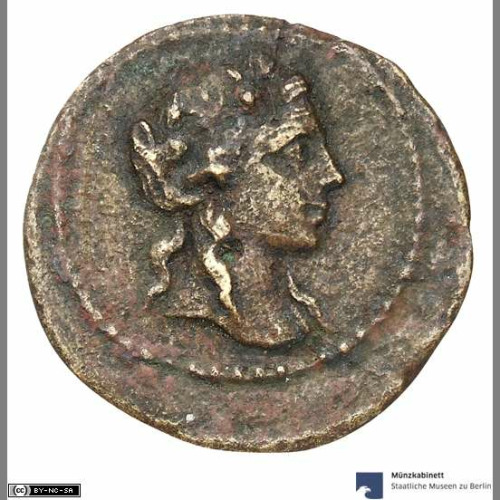
\includegraphics[width=#1]{coin3545_obverse.jpeg}}


%********************************************************************
% Bibliographies
%*******************************************************
\addbibresource{01-bibliography/references.bib}
\addbibresource[label=publications]{01-bibliography/publications.bib}
\addbibresource[label=supervision]{01-bibliography/supervisedtheses.bib}

%********************************************************************
% Hyphenation
%*******************************************************
% !TeX root = ../Thesis.tex

\hyphenation{
Si-mu-link
OO-WARP-Lab
WARP-Lab
}


%********************************************************************
% Acronyms
%*******************************************************
% !TeX root = ../Thesis.tex

\newacronym{(S+N)/NR}{(S+N)/NR}{signal-plus-noise-to-noise ratio}
\newacronym{ADC}{ADC}{analog-to-digital converter}
\newacronym{BCI}{BCI}{bulk current injection}
\newacronym{CAN}{CAN}{control area network}
\newacronym{CRT}{CRT}{cathode ray tube}
\newacronym{CSMACD}{CSMA/CD}{carrier sense multiple access with collision detection}
\newacronym{CoE}{CoE}{CAN over Ethernet}
\newacronym{DAC}{DAC}{digital-to-analog converter}
\newacronym{DoS}{DoS}{denial of service}
\newacronym{EMR}{EMR}{electromagnetic radiation}
\newacronym{FCS}{FCS}{frame check sum}
\newacronym{FEC}{FEC}{forward error correction}
\newacronym{FPGA}{FPGA}{field-programmable gate array}
\newacronym{ICMP}{ICMP}{Internet control message protocol}
\newacronym{IEC}{IEC}{International Electrotechnical Commission}
\newacronym{MAC}{MAC}{Medium Access Control}
\newacronym{NIC}{NIC}{network interface card}
\newacronym{NSA}{NSA}{National Security Agency}
\newacronym{PA}{PA}{power amplifier}
\newacronym{PC}{PC}{personal computer}
\newacronym{RF}{RF}{radio frequency}
\newacronym{SDR}{SDR}{software-defined radio}
\newacronym{SFD}{SFD}{start frame delimiter}
\newacronym{SNR}{SNR}{signal-to-noise ratio}
\newacronym{USRP}{USRP}{Universal Software Radio Peripheral}


%********************************************************************
% GO!GO!GO! MOVE IT!
%*******************************************************
\begin{document}
\frenchspacing            % no extra space after sentences
\raggedbottom             % do not stretch pages to equal height
\selectlanguage{ngerman} % the main language of the document (american, ngerman, ...)
\pagenumbering{roman}     % switch to roman (I, II, III) page numbering
\pagestyle{plain}         % show page numbers but no chapter headers on consecutive pages

%********************************************************************
% Frontmatter
%*******************************************************

% optionally group the front matter below a bookmark
\iftoggle{cts@parts}{
	\nottoggle{cts@hidefrontbackmatter}{
		\pdfbookmark[-1]{Front Matter}{frontmatter}
	}{}
}{}

\iftoggle{cts@phd}{
	% !TeX root = ../Thesis.tex

% Vorgaben zum Titelblatt einer Dissertation: https://www.intern.tu-darmstadt.de/media/dezernat_ii/promotionen_dokumente/Dissertation-Titelblatt.de.pdf

%*******************************************************
% Titlepage
%*******************************************************
\pdfbookmark[0]{\titlepagetype}{titlepage}
\begin{titlepage}
    \begin{addmargin}[-\titlePageShift]{\titlePageShift}
    \begin{center}
    \begin{otherlanguage}{ngerman}
        \large

        \includegraphics[width=6cm]{graphics/logos/tud-logo-rgb}

        \vfill

        \begingroup
            \color{CTtitle}\spacedallcaps{\myTitle} \\ \bigskip
        \endgroup

        \vfill

        Am \myFacultyDE \\
        der Technischen Universität Darmstadt \\
        eingereichte

        % -- TemplateKnob
        %% Use this for the final version:
        % Vom \myFacultyDE \\
        % der Technischen Universität Darmstadt \\
        % genehmigte

        \vspace{2ex}

        \spacedlowsmallcaps{Dissertation}

        \vspace{2ex}

        zur Erlangung des akademischen Grades \\
        \myDegreePhD \\
        von

        \vspace{2ex}

        \spacedlowsmallcaps{\myName}

        \vfill

        \begin{tabular}{r@{~}l}
        Erstreferent: & \myProf \\
        Korreferent: & \myOtherProf \\
        \end{tabular}

        \vfill

        \myLocation \DTMfetchyear{myDisputationDate} \\
        Hochschulkennziffer \myUniKennziffer

        \vfill

        \includegraphics[width=5cm]{graphics/logos/seemoo-logo-rgb} \\

    \end{otherlanguage}
    \end{center}
    \end{addmargin}
\end{titlepage}

	% !TeX root = ../Thesis.tex

% Vorgaben zum Titelblatt einer Dissertation: https://www.intern.tu-darmstadt.de/media/dezernat_ii/promotionen_dokumente/Dissertation-Titelblatt.de.pdf

\thispagestyle{empty}

\ \vfill

\noindent%
\myName, \emph{\myTitle}, Dissertation, \myLocation, \myUni, \DTMfetchyear{mySubmissionDate}.

\bigskip

\begin{otherlanguage}{ngerman}

\noindent%
\myDepartmentDE \\
\myFacultyDE \\
\myUni \\
Jahr der Veröffentlichung: \DTMfetchyear{mySubmissionDate} auf TUprints \\
Tag der mündlichen Prüfung: \DTMusedate{myDisputationDate} \\
URN: \shorturl{https://nbn-resolving.org/\myURN}{\myURN} \\

\bigskip

\noindent%
% -- TemplateKnob
% Choose the logos based on your desired CC license.

\includegraphics[height=4ex]{graphics/logos/creativecommons/cc.xlarge}

\includegraphics[height=4ex]{graphics/logos/creativecommons/by.xlarge}

\includegraphics[height=4ex]{graphics/logos/creativecommons/sa.xlarge}
% 
\includegraphics[height=4ex]{graphics/logos/creativecommons/nc-eu.xlarge}
% 
\includegraphics[height=4ex]{graphics/logos/creativecommons/nc-jp.xlarge}
% 
\includegraphics[height=4ex]{graphics/logos/creativecommons/nc.xlarge}
% 
\includegraphics[height=4ex]{graphics/logos/creativecommons/nd.xlarge}
% 
\includegraphics[height=4ex]{graphics/logos/creativecommons/pd.xlarge}
% 
\includegraphics[height=4ex]{graphics/logos/creativecommons/remix.xlarge}
% 
\includegraphics[height=4ex]{graphics/logos/creativecommons/share.xlarge}
% 
\includegraphics[height=4ex]{graphics/logos/creativecommons/zero.xlarge}

\smallskip

\noindent%
Veröffentlicht unter \emph{CC BY-SA 4.0 International}
\emph{(Namensnennung -- Weitergabe unter gleichen Bedingungen)} \\
\url{https://creativecommons.org/licenses/by-sa/4.0/deed.de}

\end{otherlanguage}

\smallskip

\noindent%
Licensed under \emph{CC BY-SA 4.0 International}
\emph{(Attribution-ShareAlike)} \\
\url{https://creativecommons.org/licenses/by-sa/4.0/deed.en}

	\cleardoublepage
	% !TeX root = ../Thesis.tex

%*******************************************************
% Dedication
%*******************************************************
\thispagestyle{empty}
\phantomsection
% -- TemplateKnob
%\addcontentsline{toc}{chapter}{\texorpdfstring{Dedication}{Dedication}}%
\pdfbookmark[0]{Dedication}{Dedication} % Create only PDF bookmark, but no TOC entry

\vspace*{3cm}

\begin{center}
    \emph{Ohana} means family. \\
    Family means nobody gets left behind, or forgotten. \\ \medskip
    --- Lilo \& Stitch
\end{center}

\medskip

\begin{center}
    Dedicated to the loving memory of Rudolf Miede. \\ \smallskip
    1939\,--\,2005
\end{center}

}{
	% !TeX root = ../Thesis.tex

%*******************************************************
% Titlepage
%*******************************************************
\pdfbookmark[0]{\titlepagetype}{titlepage}
\begin{titlepage}
	\begin{addmargin}[-\titlePageShift]{\titlePageShift}
		\begin{center}
			\large

			\includegraphics[width=6cm]{graphics/logos/goethe-logo}

			\vfill

			\begingroup
			\color{CTtitle}\spacedallcaps{\myTitle} \\ \bigskip
			\endgroup

			\vspace{2ex}

			\spacedlowsmallcaps{\myName}

			\vfill

			\myDegree

			\vspace{2ex}

			\DTMusedate{mySubmissionDate}

			\vfill

			\myDepartmentDE\\
			\myFacultyDE\\
			\myUni\\

			\vfill
		\end{center}
	\end{addmargin}
\end{titlepage}

	% !TeX root = ../Thesis.tex

\thispagestyle{empty}

\ \vfill

\noindent%
\myName, \emph{\myTitle}, \myDegree, \myUni, \DTMfetchyear{mySubmissionDate}.

\bigskip

\noindent
Abgabedatum: \DTMusedate{mySubmissionDate}

\bigskip

\noindent\begin{tabular}{@{}l@{~}l@{}}
	Betreuung: & \myProf, \mySupervisor \\
	Erstgutachter: & \myProf \\
	Zweitgutachter: & \myOtherProf
\end{tabular}

\bigskip

\noindent%
\myDepartmentDE \\
\myFacultyDE \\
\myUni


% -- TemplateKnob
% \bigskip

% \noindent%
%% Choose the logos based on your desired CC license.
% \includegraphics[height=4ex]{graphics/logos/creativecommons/cc}
% \includegraphics[height=4ex]{graphics/logos/creativecommons/by}
% \includegraphics[height=4ex]{graphics/logos/creativecommons/sa}
%% \includegraphics[height=4ex]{graphics/logos/creativecommons/nc}
%% \includegraphics[height=4ex]{graphics/logos/creativecommons/nd}

% \smallskip

% \begin{otherlanguage}{ngerman}

% \noindent%
% Veröffentlicht unter \emph{CC BY-SA 4.0 International}
% \emph{(Namensnennung -- Weitergabe unter gleichen Bedingungen)} \\
% \url{https://creativecommons.org/licenses/by-sa/4.0/deed.de}

% \end{otherlanguage}

% \smallskip

% \noindent%
% Licensed under \emph{CC BY-SA 4.0 International}
% \emph{(Attribution-ShareAlike)} \\
% \url{https://creativecommons.org/licenses/by-sa/4.0/deed.en}

}

\cleardoublepage
% !TeX root = ../Thesis.tex

%*******************************************************
% Abstract
%*******************************************************

\iftoggle{cts@phd}{%
\begingroup
\let\clearpage\relax
\let\cleardoublepage\relax
\let\cleardoublepage\relax
}{}

\addchapCondToC{Abstract}
Diese Arbeit untersucht, ob sich einzelne visuelle Merkmale auf antiken Münzbildern ohne münzspezifisches Training detektieren und für den Vergleich von Münzen nutzen lassen. Manuelle Stempelstudien sind sehr aufwendig, und bestehende bildbasierte Verfahren erfordern meist ein Training auf münzspezifischen Daten.
Für die Detektion wird das Open-Vocabulary-Modell YOLO-World eingesetzt, das Merkmale im Zero-Shot-Verfahren anhand von Textbeschreibungen erkennt. Zu jedem detektierten Merkmal wird ein Feature-Vektor aus einer internen Schicht des Netzwerks extrahiert. Merkmale derselben Klasse auf verschiedenen Münzen werden mit euklidischer Distanz, Manhattan-Distanz und Kosinus-Ähnlichkeit verglichen. Die Umsetzung erfolgt als Anwendung, die Verarbeitung, Speicherung und Suche ermöglicht.
Die Auswertung nutzt 200 Münzen aus dem Corpus Nummorum in 20 Stempelgruppen zu je zehn Münzen als Grundwahrheit. Geprüft wird, ob Münzen mit demselben Vorderseitenstempel unter den ähnlichsten Treffern liegen (HitRate@1, HitRate@5, Precision@5). YOLO-World liefert bei einem Schwellenwert von 0{,}005 auf den Vorderseiten 905 Detektionen mit meist niedriger Confidence, nur 23 der 57 Prompts treten als Klasse auf. Über alle Klassen liegt bei 30,8\,\% der Anfragen eine Münze desselben Stempels unter den fünf ähnlichsten Treffern, bei zufälliger Reihenfolge wären es 21,2\,\%. Deutlich über dem Zufall liegen nur Gesichter (\textit{human face}: 42,0\,\% gegenüber 20,9\,\%), bei anderen Klassen trennen die Vektoren nicht. Da auf Münzen desselben Stempels oft verschiedene Klassen detektiert werden, bleiben viele stempelgleiche Münzen unverglichen. Das ohne Open Vocabulary arbeitende YOLOv8n erreicht vergleichbare Werte. Grenzen ergeben sich aus der Abhängigkeit von der Prompt-Liste, der kleinen Datenbasis und dem Erhaltungszustand der Münzen.

\iftoggle{cts@phd}{%
\vfill
\begin{otherlanguage}{ngerman}
  \addchapCondToC{Zusammenfassung}
  Kurze Zusammenfassung des Inhaltes in deutscher Sprache\dots
  \lipsum[11-20][1-12]
\end{otherlanguage}
\endgroup
\vfill
}{}

\cleardoublepage
% !TeX root = ../Thesis.tex

%*******************************************************
% Acknowledgments
%*******************************************************
\bigskip

\begingroup
\let\clearpage\relax
\let\cleardoublepage\relax
\let\cleardoublepage\relax

% -- TemplateKnob - pick your acknowledgement style and adapt it to your liking

% ------------------------------------------------------------------------------
% Standard acknowledgements
% - with chapter heading
% ------------------------------------------------------------------------------
%\addchapCondToC{Acknowledgments}
%{\slshape
%{\slshape
%Unser Dank gilt zuerst \myProf für die Betreuung dieser Arbeit und für die Möglichkeit, ein Thema an der Schnittstelle von Informatik und Numismatik zu bearbeiten. Ebenso danken wir \mySupervisor für die engagierte Begleitung, die fachlichen Anregungen und die Zeit, die er sich für unsere Fragen genommen hat. Herrn \myOtherProf danken wir für die Übernahme des Zweitgutachtens.
%
%\bigskip
%
%Bedanken möchten wir uns auch bei allen, die diese Arbeit Korrektur gelesen haben: Ahmed Kaid, Sofia Liben, Eva Kaufholz-Soldat, Marit Haußmann. Eure Hinweise zu Inhalt, Aufbau und Sprache haben den Text deutlich verbessert, und jeder verbleibende Fehler geht allein auf uns.
%
%
%}
%}
% ------------------------------------------------------------------------------


% ------------------------------------------------------------------------------
% Simple acknowledgements
% - no chapter heading
% - placed on page according to golden ratio :)
% - consider also: centering, leaving out the headline, adding a fun emoji
% ------------------------------------------------------------------------------
\phantomchapCondToC{Acknowledgments}
\begin{vplace}[0.618]
{\slshape
Unser Dank gilt zuerst \myProf für die Betreuung dieser Arbeit und für die Möglichkeit, ein Thema an der Schnittstelle von Informatik und Numismatik zu bearbeiten. Ihm und \mySupervisor danken wir für die engagierte Begleitung, die fachlichen Anregungen und die Zeit, die er sich für unsere Fragen genommen hat. Herrn \myOtherProf danken wir für die Übernahme des Zweitgutachtens.

\bigskip

Bedanken möchten wir uns auch bei allen, die diese Arbeit Korrektur gelesen haben: Ahmed Kaid, Sofia Liben, Eva Kaufholz-Soldat und Marit Haußmann. Eure Hinweise zu Inhalt, Aufbau und Sprache haben den Text deutlich verbessert, und jeder verbleibende Fehler geht allein auf uns.
}
\end{vplace}
% ------------------------------------------------------------------------------

\endgroup


% show page numbers and chapter headings on consecutive pages
\pagestyle{scrheadings}

\cleardoublepage
% !TeX root = ../Thesis.tex

%*******************************************************
% Table of Contents
%*******************************************************
\pdfbookmark[0]{\contentsname}{tableofcontents}
\setcounter{tocdepth}{2} % <-- 2 includes up to subsections in the ToC
\setcounter{secnumdepth}{3} % <-- 3 numbers up to subsubsections
\manualmark
\markboth{\spacedlowsmallcaps{\contentsname}}{\spacedlowsmallcaps{\contentsname}}
\tableofcontents
\automark[section]{chapter}
\renewcommand{\chaptermark}[1]{\markboth{\spacedlowsmallcaps{#1}}{\spacedlowsmallcaps{#1}}}
\renewcommand{\sectionmark}[1]{\markright{\textsc{\thesection}\enspace\spacedlowsmallcaps{#1}}}
%*******************************************************
% List of Figures and of the Tables
%*******************************************************
\clearpage
\begingroup
\let\clearpage\relax
\let\cleardoublepage\relax
%*******************************************************
% List of Figures
%*******************************************************
\phantomchapCondToC{\listfigurename}
\listoffigures

\vspace{8ex}

%*******************************************************
% List of Tables
%*******************************************************
\phantomchapCondToC{\listtablename}
\listoftables

\vspace{8ex}
% \newpage

% %*******************************************************
% % List of Listings
% %*******************************************************
% % Change the listing caption to "Quelltext"
% \renewcommand{\lstlistingname}{Quelltext}
% \phantomchapCondToC{\lstlistlistingname}
% \lstlistoflistings
%
% \vspace{8ex}

%*******************************************************
% Acronyms
%*******************************************************
\phantomchapCondToC{Akronyme}
\printglossary[type=\acronymtype]

\endgroup

% add space after contents if parts are not enabled (needs to be here for LaTeX reasons)
\nottoggle{cts@parts}{\tocextraspace}{}

\iftoggle{cts@phd}{
	\cleardoublepage
	% !TeX root = ../Thesis.tex

%*******************************************************
% Publications
%*******************************************************
\addchap{List of Publications}
\label{ch:AuthorPublications}

During the course of writing this thesis, I co-authored several papers and articles that I list below.

\begin{refsection}[publications]
\nocite{*} % is local to to the enclosing refsection

% ----------------------------------------------------------------------------------------------------
%
% Suggested bibliography keywords
%
%  *  conferenceproceedings   -> conference papers
%  *  journalarticle          -> journal articles
%  *  posterdemo              -> posters and demos
%  *  extendedabstract        -> extended abstracts
%  *  underreview             -> publication currently under review
%  *  partofthesis            -> publications part of the cumulative dissertation
%  *  supervisedthesis        -> student theses (bsc/msc) supervised by the PhD student
%
% (you can filter with 'keyword' and 'notkeyword')
%
%
% ----------------------------------------------------------------------------------------------------

\section*{Publications Included in this Thesis}

\printbibliography[
  heading=none,
  keyword=mypublication,
  keyword=partofthesis,
]

\section*{Further Publications}

\printbibliography[
  heading=none,
  keyword=mypublication,
  notkeyword=partofthesis,
]



% uncomment these subsections for a more fine-grained bibliography

% \subsection*{Journal and Magazine Articles}
% \printbibliography[
%   heading=none,
%   keyword=mypublication,
%   notkeyword=partofthesis,
%   notkeyword=underreview,
%   keyword=journalarticle,
% ]



% \subsection*{Conference and Workshop Papers}
% \printbibliography[
%   heading=none,
%   keyword=mypublication,
%   notkeyword=partofthesis,
%   notkeyword=underreview,
%   keyword=conferenceproceedings
% ]



% \subsection*{Posters and Demonstrators}
% \printbibliography[
%   heading=none,
%   keyword=mypublication,
%   notkeyword=partofthesis,
%   notkeyword=underreview,
%   keyword=posterdemo
% ]



% \subsection*{Extended Abstracts}
% \printbibliography[
%   heading=none,
%   keyword=mypublication,
%   notkeyword=partofthesis,
%   notkeyword=underreview,
%   keyword=extendedabstract
% ]



% \subsection*{Under Peer Review}
% \printbibliography[
%   heading=none,
%   keyword=mypublication,
%   notkeyword=partofthesis,
%   keyword=underreview
% ]

\end{refsection}

\label{ch:AuthorPublicationsEnd}

	% -- TemplateKnob
	%\cleardoublepage
	%% !TeX root = ../Thesis.tex

%*******************************************************
% Teaching and Outreach
%*******************************************************
\addchap{Teaching and Outreach}
\label{ch:Teaching}

This is a basic template for an extensive academic CV. Expand as you see fit.

\section*{Supervision of Student Research}
During my time at the Secure Mobile Networking Lab of TUDa, I was involved in the supervision of $n$ Master's theses, $k$ Bachelor's theses, $j$ seminars and $l$ labs.
\begin{refsection}[supervision]

% anonymize the list of supervised theses, unless your students agreed to be listed here
\renewbibmacro{author}{}

\nocite{*} % is local to to the enclosing refsection
\printbibliography[
  heading=none,
  keyword=supervisedthesis
]
\end{refsection}


\section*{Teaching Activites}

Write about lectures, tutorials, exercises, and course organization.


\section*{Scientific Outreach and Media Contributions}

Write about press activities, public talks, interviews, blog posts, podcasts, etc.
 % not required in final submission
	\cleardoublepage
	% !TeX root = ../Thesis.tex

%*******************************************************
\addchap{Collaborations and My Contributions}
%*******************************************************
\label{ch:Collaborations}

% From Daniel Steinmetzer's dissertation
Systematically investigating a technical research topic and engineering the required tools is a demanding and interdisciplinary process. Most achievements could never evolve without collaborations in which colleagues and international partners integrated their intellectual forces. When working in teams, accounting particular contributions and components of the resulting publications to individual collaborators becomes almost impossible. This situation also applies to several contents of this thesis, which arise from collaborations, thus, cover joint contributions. Many of these collaborations persisted even longer than the research projects and became a long-term strategic partnership.
In our previous publications, all authors contributed by discussing ideas and debating on results throughout the whole project duration. Each of them has particular strengths that sometimes appear invisible. For this reason, I explicitly state and acknowledge---where possible---the contributions of my collaborators in the following.

% From Milan Stute's dissertation
In the following, I detail the contributions of my co-authors and myself per chapter. In addition, I follow the regulations of the \myFaculty at \myUni and give an account of the parts that include verbatim or revised fragments of previous publications that form this thesis as indicated in the preceding list of publications.\footnote{References in this chapter refer to my list of publications given on \cpagerefrange*{ch:AuthorPublications}{ch:AuthorPublicationsEnd}.}

\sloppy

\Cref{ch:introduction,ch:relatedwork} collate the contributions, background, and related work sections of the core papers that form this thesis.%~\cite{Stute2020}.

% etc etc etc

\fussy

\label{ch:CollaborationsEnd}

}{}

%********************************************************************
% Mainmatter
%*******************************************************
\cleardoublepage       % start the main matter on an odd numbered page (before \pagenumbering)
\pagenumbering{arabic} % switch to arabic (1, 2, 3) page numbering

\iftoggle{cts@parts}{
	\cleardoublepage % ensure that the PDF bookmark to the following part points to the right page
	%\ctparttext{Description of the first part.} % -- TemplateKnob (adjust or leave it)
	\part{Introduction}
}{}

% !TeX root = ../Thesis.tex

%************************************************
\chapter{Einleitung}\label{ch:introduction}
%************************************************
\glsresetall % Resets all acronyms to not used

%**********Motivation und Kontext*************
\section{Motivation und Kontext}
\label{sec:firstsection}
Antike Münzen wurden mit handgefertigten Stempeln geprägt (vgl. \cref{sec:glnumismatik}). Münzen desselben Stempels sollten sich daher besonders ähnlich sein, und aus den Kombinationen der Stempel lässt sich die Reihenfolge der Prägung rekonstruieren \cite{wikipedia-numismatik}. Manuelle Stempelstudien sind jedoch so aufwendig, dass große Prägungen, etwa die des Römischen Reichs, kaum umfassend untersucht werden können \cite{heinecke2021unsupervised}. \todo{Rückfrage: Soll hier ein Beleg stehen, dass Stempelvergleiche eine etablierte Methode sind (z. B. Kluge, Howgego)?} Digitale Datenbanken wie das Corpus Nummorum \cite{peter2024corpus} stellen große Mengen an Münzbildern bereit (vgl. \cref{sec:gesamtansatzdatengrundlage}). Bildbasierte Verfahren wurden für antike Münzen bereits eingesetzt, etwa zur Zuordnung von Münzen zu ihrer Prägung (engl. Issue) \cite{guo2023siamese}, zur Erkennung einzelner Motive wie Adler oder Schild \cite{cooper2020learning}, zur Zeichenerkennung auf Legenden \cite{anwar2026reading} und zur Automatisierung der Stempelanalyse \cite{heinecke2021unsupervised}. Mehrere dieser Verfahren erfordern ein Training auf münzspezifischen Daten \cite{guo2023siamese,cooper2020learning,anwar2026reading}.

Die vorliegende Arbeit untersucht, ob sich einzelne Merkmale auf antiken Münzbildern auch ohne münzspezifisches Training detektieren und für einen Vergleich nutzen lassen. Entscheidend ist dabei nicht, ob ein detektiertes Merkmal inhaltlich korrekt benannt wird, sondern ob Merkmale derselben Klasse, die auf verschiedenen Münzen detektiert werden, miteinander verglichen werden können. Eine ausführliche Einordnung in bestehende Arbeiten folgt in \cref{sec:bestehendearbeiten}.


%**********Zielsetzung und Forschungsfragen*************
\section{Zielsetzung und Forschungsfragen}
\label{sec:zielsetzungundforschungsfragen}
Ziel der vorliegenden Arbeit ist es, visuelle Merkmale auf antiken Münzbildern mithilfe eines YOLO-Modells (zu erkennen und) zu lokalisieren und anschließend anhand ihrer extrahierten Feature-Vektoren miteinander zu vergleichen.
Im Rahmen der Recherche wurde kein Modell gefunden, das für die Detektion der hier betrachteten Merkmale auf antiken Münzbildern trainiert wurde \todo{Formulierung prüfen, siehe Anmerkung} (vgl. \cref{sec:modelle}). Ein eigenes Training würde zudem Annotationen der Merkmalspositionen voraussetzen, die nicht vorliegen. Deshalb wird bewusst ein Ansatz ohne Nachtraining verfolgt. Untersucht wird dabei, inwieweit sich ein nicht auf Münzen angepasstes Modell für die Detektion und den Vergleich von Merkmalen auf antiken Münzbildern eignet.
Aus dieser Zielsetzung ergeben sich folgende Forschungsfragen:
\begin{enumerate}
    \item Inwieweit lassen sich visuelle Merkmale auf antiken Münzbildern mithilfe eines nicht speziell trainierten YOLO-Modells detektieren und lokalisieren?
    \item Inwiefern lassen sich lokalisierte Merkmale anhand ihrer extrahierten Feature-Vektoren sinnvoll miteinander vergleichen?
    \item Welche Grenzen zeigt ein Ansatz ohne münzspezifisches Training bei der Anwendung auf antike Münzbilder?
\end{enumerate}

\noindent Nicht Gegenstand der Arbeit sind das Training oder Nachtrainieren eigener Modelle sowie die numismatische Bestimmung oder Datierung von Münzen. Der Vergleich ganzer Münzbilder ist in der Anwendung als ergänzende Funktion umgesetzt, wird aber nicht untersucht (vgl. \cref{sec:gesamtansatzdatengrundlage}).
% !TeX root = ../Thesis.tex

%************************************************
\chapter{Grundlagen}\label{ch:grundlagen}
%************************************************
\glsresetall % Resets all acronyms to not used

%**********Grundlagen der Numismatik*************
\section{Grundlagen der Numismatik}
\label{sec:glnumismatik}
Die Numismatik, auch Münzkunde genannt, beschäftigt sich mit der wissenschaftlichen Analyse von Münzen und dem Geldwesen. Sie berührt dabei unter anderem die Archäologie sowie die Geschichts-, Wirtschafts- und Sozialwissenschaft \cite{wikipedia-numismatik}. Im Mittelpunkt dieser Arbeit stehen antike Münzen, genauer ihre Münzbilder, als Untersuchungsgegenstand.

Aus vielen Epochen und Regionen sind Münzfunde und Sammlungen erhalten, so stammen die ältesten Münzen aus der Zeit um 600 v. Chr. \cite{vonkaenel2012ersten}. Als historische Quellen geben Münzen Auskunft über die Zeit, in der sie geprägt und im Handel genutzt wurden. Daraus lassen sich somit politische und wirtschaftliche Entwicklungen nachvollziehen. Da Münzen in großer Zahl erhalten sind, sind sie besonders für Epochen von Interesse, aus denen wenig schriftliche Überlieferung oder wenige genaue Datierungen vorliegen. Ihre Prägungen zeigen Datierungshinweise und Inschriften sowie Darstellungen von Personen und Symbolen, die auf Zeit und Kultur der Prägung verweisen. Auf antiken Münzen sind etwa Gottheiten und Heroen wie Herakles, Aphrodite oder Athena abgebildet. Die Römer übernahmen viele Motive von den Griechen, die bereits Personen darstellten. Eine Besonderheit römischer Münzen sind Abbildungen von Herrschern; Caesar war der erste Römer, der zu Lebzeiten auf einer Münze abgebildet wurde \cite{howgego1995ancient,museumdigital-roemische-muenzen} \todo{Formulierung und Seite prüfen}. 

Antike Münzen werden in Vorder- und Rückseite unterteilt, die als Obverse (auch Avers) und Reverse (auch Revers) bezeichnet werden. Bei römischen Kaisermünzen zeigt die Vorderseite in der Regel die Büste des Herrschers, die Rückseite dagegen Verschiedenes, beispielsweise das Bild einer Gottheit, Insignien, Tiere oder Gegenstände \cite{museumdigital-roemische-muenzen}. Zusätzlich trägt die Vorderseite häufig eine Legende, also eine Inschrift mit Namen, Titeln oder weiteren Angaben \cite{cooper2020learning}, siehe \cref{fig:coin-3545}. Andere antike Prägungen weichen davon ab. Frühe thrakische Münzen zeigen auf der Vorderseite häufig ein Tier oder einen Gegenstand und auf der Rückseite ein vertieftes Viereck (Quadratum Incusum) \cite{berthold2016thrakien}. Welche Motive im Datensatz dieser Arbeit vorkommen, wird in \cref{sec:gesamtansatzdatengrundlage} beschrieben. Diese sichtbaren und inhaltlich interpretierbaren Bestandteile werden in dieser Arbeit als visuelle Merkmale bezeichnet (vgl. \cref{sec:merkmale}).

\begin{figure}[H]
    \centering

    \begin{subfigure}{0.4\textwidth}
        \centering
        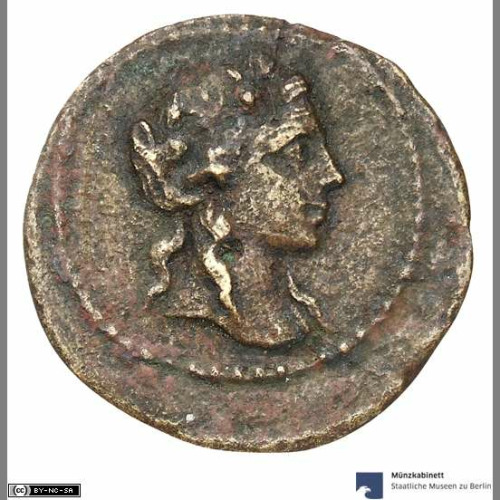
\includegraphics[width=\textwidth]{coin3545_obverse.jpeg}
        \caption{Vorderseite}
    \end{subfigure}
    \hspace{0.04\textwidth}
    \begin{subfigure}{0.4\textwidth}
        \centering
        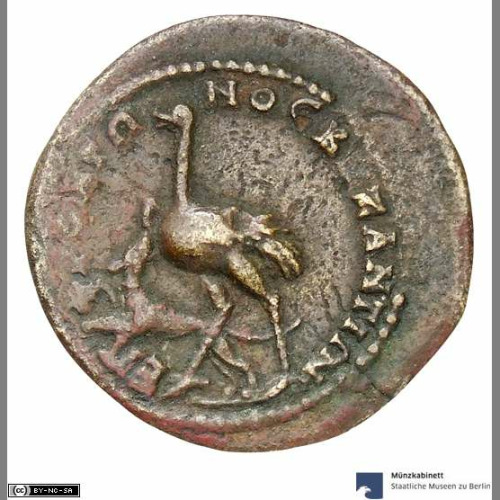
\includegraphics[width=\textwidth]{coin3545_reverse.jpeg}
        \caption{Rückseite}
    \end{subfigure}

    \caption[Beispielmünze aus dem Corpus Nummorum] {Beispielmünze aus dem Corpus Nummorum. Ca. 222-235 n. Chr. Münzstätte Byzantion, Region Thrakien.
  Quelle: cn coin 3545 \cite{cn-coin-3545}. Original, Münzkabinett, Staatliche Museen
  zu Berlin, Inv.-Nr.~18235544. Foto: Reinhard Saczewski. Lizenz: Public Domain Mark 1.0.}
    \label{fig:coin-3545}
\end{figure}

\noindent Auch die Herstellung beeinflusst das Erscheinungsbild. Münzen wurden von der Antike bis in die frühe Neuzeit durch Hammerprägung hergestellt \cite{wikipedia-muenzpraegung}. Ein Münzrohling, der sogenannte Schrötling, wurde auf einen fest installierten Unterstempel gelegt, der das Motiv der Vorderseite trug. Ein frei geführter Oberstempel mit dem Motiv der Rückseite wurde daraufgesetzt und mit einem Hammerschlag eingeprägt, sodass beide Seiten geprägt wurden \cite{adfontes-herstellung}. Da jeder Stempel ein in Handarbeit gefertigtes Einzelstück war, unterscheiden sich auch Münzen desselben Typs in feinen Details \cite{wikipedia-muenzpraegung}. Außerdem nutzten sich die Stempel ab und mussten ersetzt werden, wobei der Oberstempel in der Regel früher ausgetauscht wurde als der Unterstempel. Dadurch ergeben sich unterschiedliche Stempelkombinationen, anhand derer sich die Reihenfolge der Prägung rekonstruieren lässt (Stempelanalyse) \cite{wikipedia-numismatik}.

Zusätzlich verändert sich das Erscheinungsbild im Laufe der Objektgeschichte \cite{wikipedia-numismatik}. Nutzung und Umlauf führen zu Abnutzung, die je nach Erhaltungsgrad unterschiedlich stark ausfällt \cite{wikipedia-erhaltungsgrade,adfontes-abnutzung} (\cref{fig:erhaltung}). Bei Münzen, die lange im Boden lagen, kann je nach Bodenbedingungen außerdem das Metall korrodieren. Motive, Symbole und Legenden können dadurch teilweise oder vollständig unkenntlich werden \cite{adfontes-abnutzung}. Abnutzung und Korrosion erschweren zudem die automatisierte Erkennung von Merkmalen auf antiken Münzbildern, da Details und Legenden verloren gehen \cite{fare2017ancient,heinecke2021unsupervised} (vgl. \cref{sec:modelle}).

\begin{figure}[H]
    \centering

    \begin{subfigure}{0.4\textwidth}
        \centering
        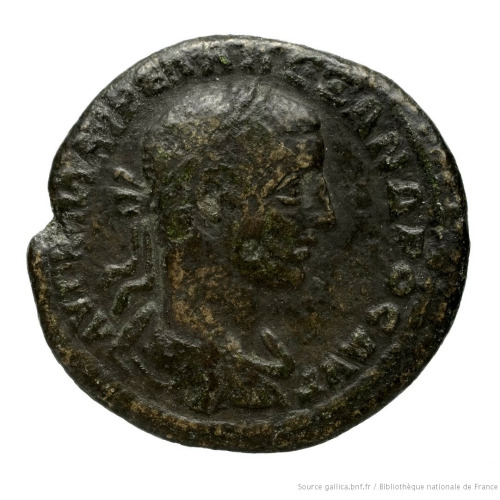
\includegraphics[width=\textwidth]{coin1018_obverse.jpeg}
        \caption{Original}
        \label{fig:originalcoin1018}
    \end{subfigure}
    \hspace{0.04\textwidth}
    \begin{subfigure}{0.4\textwidth}
        \centering
        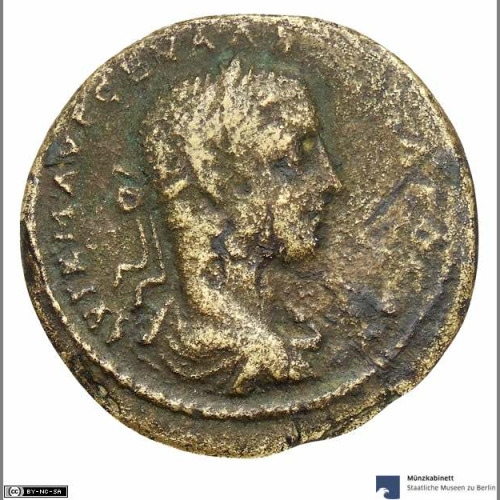
\includegraphics[width=\textwidth]{coin1019_obverse.jpeg}
        \caption{Original}
        \label{fig:originalcoin1019}
    \end{subfigure}

    \vspace{0.6em}

    \begin{subfigure}{0.4\textwidth}
        \centering
        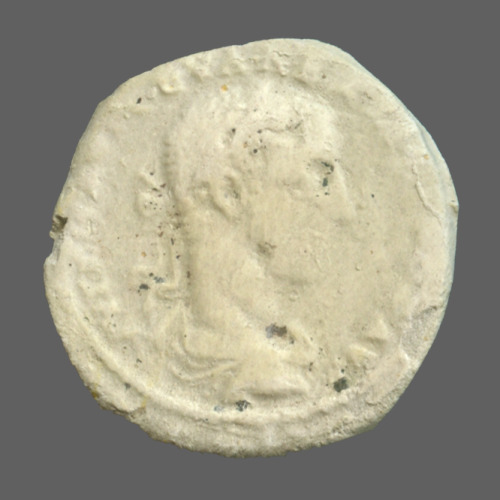
\includegraphics[width=\textwidth]{coin1015_obverse.jpeg}
        \caption{Gipsabguss}
        \label{fig:gibsabgusscoin1015}
    \end{subfigure}
    \hspace{0.04\textwidth}
    \begin{subfigure}{0.4\textwidth}
        \centering
        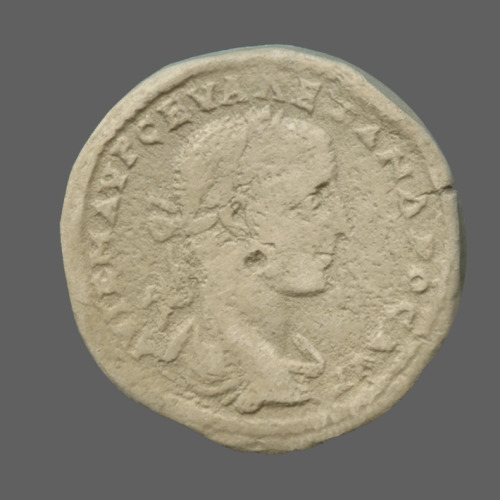
\includegraphics[width=\textwidth]{coin1017_obverse.jpeg}
        \caption{Gipsabguss}
        \label{fig:gipsabgusscoin1017}
    \end{subfigure}
    \caption[Münzen in unterschiedlichem Erhaltungszustand]{Münzen aus dem Corpus Nummorum in unterschiedlichem Erhaltungszustand, alle aus Byzantion, Region Thrakien, ca. 222--235 n.~Chr.: Originale (oben) und Gipsabgüsse (unten).
    (a) cn coin 1019~\cite{cn-coin-1019}. Original, Münzkabinett, Staatliche Museen zu Berlin, Inv.-Nr.~18235900. Foto: Reinhard Saczewski. Lizenz: Public Domain Mark 1.0.
    (b) cn coin 1018~\cite{cn-coin-1018}. Original, Bibliothèque nationale de France, Département des Monnaies, médailles et antiques, Paris, Inv.-Nr.~466. Lizenz: CC BY-NC-SA 4.0.
    (c) cn coin 1017~\cite{cn-coin-1017}. Gipsabguss. Foto: BBAW. Lizenz: CC BY-NC-SA 4.0.
    (d) cn coin 1015~\cite{cn-coin-1015}. Gipsabguss. Foto: BBAW. Lizenz: CC BY-NC-SA 4.0.}
    \label{fig:erhaltung}
\end{figure}

%**********Grundlagen des maschinellen Lernens*************
\section{Grundlagen des maschinellen Lernens}
\label{sec:glmaschinelleslernen}
Die technische Grundlage dieser Arbeit bildet das maschinelle Lernen, ein Teilgebiet der künstlichen Intelligenz. Im Gegensatz zu regelbasierten Verfahren wird der Lösungsweg nicht vollständig vorgegeben. Ein Modell wird anhand von Beispieldaten trainiert und kann anschließend auch für unbekannte Daten Vorhersagen treffen \cite{goodfellow2016deep,lecun2015deep} \todo{Goodfellow: Kap.5 (Learning Algorithms, Generalisierung) Seiten?}. 
Beim überwachten Lernen (Supervised Learning) stehen im Training zu den Eingabedaten die erwarteten Ausgaben zur Verfügung, etwa Bilder mit zugeordneter Klasse. Beim unüberwachten Lernen fehlen solche Zielwerte \cite{goodfellow2016deep,lecun2015deep}. Da Objektdetektoren in der Regel überwacht trainiert werden (vgl. \cref{sec:ooyolo}), ist für diese Arbeit das überwachte Lernen maßgeblich. 

Eine Weiterentwicklung stellt das Deep Learning dar, dessen Grundlage künstliche neuronale Netze sind. Ein solches Netz besteht aus mehreren hintereinandergeschalteten Schichten, nämlich: einer Eingabeschicht, einer oder mehreren verdeckten Schichten (Hidden Layers) und einer Ausgabeschicht \cref{fig:nn}. 

\begin{figure}[H]
  \centering
  \resizebox{0.7\linewidth}{!}{\begin{tikzpicture}[x=1cm,y=1cm]
  % Netz 4-4-4-2 (nur Aufbau: Schichten und Verbindungen)
  \foreach \l/\n/\col in {0/4/figblue!20,1/4/figorange!20,2/4/figorange!20,3/2/figgreen!25} {
    \foreach \i in {1,...,\n} {
      \node[figneuron, fill=\col] (n\l-\i) at (\l*1.5, {(\n+1)/2*0.8-\i*0.8}) {};
    }
  }
  \foreach \l/\m/\cnt in {0/1/4,1/2/4,2/3/2} {
    \foreach \i in {1,...,4} {
      \foreach \j in {1,...,\cnt} {
        \draw[black!35, line width=0.3pt] (n\l-\i) -- (n\m-\j);
      }
    }
  }
  \node[figlabel] at (0,-2.4) {Eingabe};
  \node[figlabel] at (2.25,-2.4) {verdeckte Schichten};
  \node[figlabel] at (4.5,-2.4) {Ausgabe};
\end{tikzpicture}
}
  \caption[Aufbau eines neuronalen Netzes]{Aufbau eines künstlichen neuronalen Netzes aus Eingabeschicht, verdeckten Schichten und Ausgabeschicht. Eigene Darstellung nach dem Prinzip aus \cite{goodfellow2016deep}.}
  \label{fig:nn}
\end{figure}

Verdeckt heißen die mittleren Schichten, weil die Trainingsdaten nur die gewünschte Ausgabe vorgeben, nicht aber, was in diesen Schichten berechnet werden soll \cite{goodfellow2016deep}. Jede Schicht erhält die Werte der vorherigen Schicht, verrechnet sie mit gewichteten Verbindungen und reicht das Ergebnis weiter. Die Gewichte bestimmen, wie stark ein Eingangswert in das Ergebnis eingeht. Durch eine Aktivierungsfunktion, in modernen Netzen meist die ReLU-Funktion, kann das Netz auch nichtlineare Zusammenhänge abbilden. Ohne sie ließe sich selbst ein Netz mit mehreren Schichten auf eine einzige lineare Abbildung zurückführen \cite{goodfellow2016deep, lecun2015deep}. Die Gewichte und die weiteren einstellbaren Größen des Netzes heißen zusammen Parameter. Sie werden im Training schrittweise angepasst. Die Ausgabe des Netzes wird mit dem erwarteten Ergebnis verglichen, und eine Kostenfunktion (Verlustfunktion, Loss Function) misst die Abweichung. Mit der Backpropagation wird berechnet, wie stark jeder Parameter zu diesem Fehler beiträgt. Dazu wird der Fehler mithilfe der Kettenregel (Kettenregel der Differentialrechnung) rückwärts durch das Netz geführt. Anhand dieser Werte werden die Parameter dann so verändert, dass der Fehler sinkt. Über viele Durchläufe durch die Trainingsdaten lernt das Netz so, welche Eigenschaften der Eingabe für die Aufgabe wichtig sind \cite{goodfellow2016deep, lecun2015deep}. Der Ablauf ist in \cref{fig:nn-training} dargestellt.

\begin{figure}[H]
  \centering
  \resizebox{\linewidth}{!}{% Optional: nur einbinden, wenn der Text Verlustfunktion und Backpropagation beschreibt
\begin{tikzpicture}
  \node[figbox, sblue] (in) at (0,0) {Eingabe};
  \node[figbox, sorange] (net) at (3,0) {Netz};
  \node[figbox, sblue] (out) at (6,0) {Ausgabe};
  \node[figbox, sorange] (loss) at (9,0) {Verlust-\\funktion};
  \node[figbox, sgreen] (exp) at (9,-1.8) {erwartetes\\Ergebnis};
  \draw[figarrow] (in) -- (net);
  \draw[figarrow] (net) -- (out);
  \draw[figarrow] (out) -- (loss);
  \draw[figarrow] (exp) -- (loss);
  \draw[figarrow, dashed] (loss.north) -- ++(0,0.8) -| (net.north)
    node[pos=0.25, above, figlabel] {Backpropagation};
\end{tikzpicture}
}
  \caption[Training eines neuronalen Netzes]{Trainingsablauf eines neuronalen Netzes: Die Ausgabe des Netzes wird mit dem erwarteten Ergebnis verglichen, die Verlustfunktion misst die Abweichung, und per Backpropagation werden die Parameter des Netzes angepasst. Eigene Darstellung nach dem Prinzip aus \cite{goodfellow2016deep,lecun2015deep}.}
  \label{fig:nn-training}
\end{figure}

\noindent Für Bilddaten haben sich Convolutional Neural Networks (CNNs) etabliert, deren Architektur auf räumlich strukturierte Daten ausgelegt ist \cite{goodfellow2016deep, lecun2015deep}. Ihr zentrales Element sind Faltungsschichten (Convolutional Layers). Sie verwenden Filter, kleine Gewichtsmatrizen, die über das Bild geschoben werden und dabei lokale Bildbereiche auf bestimmte Strukturen untersuchen (\cref{fig:faltung}). Derselbe Filter wird dabei an allen Bildpositionen verwendet, sodass das Netz weniger Parameter benötigt \cite{goodfellow2016deep}. 

\begin{figure}[H]
  \centering
  \resizebox{\linewidth}{!}{\begin{tikzpicture}[x=0.6cm,y=0.6cm, every node/.style={font=\small}]
  % Eingabe 5x5: Zeilen "0 0 9 9 9"
  \foreach \r in {0,...,4}{
    \foreach \c/\v/\g in {0/0/0,1/0/0,2/9/27,3/9/27,4/9/27}{
      \node[draw=black!50, minimum size=0.6cm, inner sep=0pt, fill=black!\g] at (\c,-\r) {\v};
    }
  }
  % Hervorgehobener Ausschnitt (Zeilen/Spalten 1-3 -> Index 0..2)
  \draw[figblue, line width=1.6pt] (-0.5,0.5) rectangle (2.5,-2.5);
  \node[figlabel] at (2,1.2) {Bildausschnitt (5$\times$5)};

  \node at (5.1,-1) {$\ast$};
  % Kernel
  \foreach \r in {0,1,2}{
    \foreach \c/\v in {0/1,1/0,2/-1}{
      \node[draw=figorange, fill=figorange!15, minimum size=0.6cm, inner sep=0pt] at (6.2+\c,-0.0-\r-0) {\v};
    }
  }
  \node[figlabel] at (7.2,1.2) {Filter (3$\times$3)};
  \node at (10.3,-1) {$=$};
  % Ausgabe 3x3: je Zeile -27 -27 0
  \foreach \r in {0,1,2}{
    \foreach \c/\v in {0/-27,1/-27,2/0}{
      \node[draw=black!50, minimum size=0.6cm, inner sep=0pt, fill=figgreen!15] at (11.4+\c,-\r) {\v};
    }
  }
  \draw[figblue, line width=1.6pt] (10.9,0.5) rectangle (11.9,-0.5);
  \node[figlabel] at (12.4,1.2) {Ergebnis (3$\times$3)};
  \node[figlabel, text width=7cm] at (6.5,-5.6) {Beispiel: $3\cdot(0\cdot1+0\cdot0+9\cdot(-1)) = -27$\\(großer Betrag bei einer senkrechten Kante)};
\end{tikzpicture}
}
  \caption[Faltung mit einem Filter]{Funktionsprinzip eines Filters in einer Faltungsschicht: Der Filter wird über den Bildausschnitt geschoben, und an jeder Position werden die Produkte aus Bild- und Filterwerten summiert. Der markierte Ausschnitt ergibt $3\cdot(0\cdot1+0\cdot0+9\cdot(-1))=-27$, der Betrag ist bei der senkrechten Kante groß. Eigene Darstellung mit beispielhaft gewählten Zahlenwerten.}
  \label{fig:faltung}
\end{figure}

\noindent Frühe Schichten erfassen einfache Strukturen wie Kanten, spätere setzen diese zu komplexeren Mustern und Formen zusammen. So entsteht eine hierarchische Repräsentation des Bildes. Anders als bei klassischen Verfahren der Bildverarbeitung müssen die relevanten Merkmale dabei nicht manuell festgelegt werden, sondern werden aus den Trainingsdaten erlernt \cite{lecun2015deep, goodfellow2016deep}. Pooling-Schichten fassen benachbarte Werte zusammen, beispielsweise über den Maximalwert oder den Durchschnitt, und verkleinern so die räumliche Auflösung der Merkmalskarten \cite{goodfellow2016deep}. 

\noindent Ein Modell muss nicht für jede Aufgabe von Grund auf trainiert werden. Beim Transfer Learning werden Repräsentationen, die ein Modell auf einem großen, allgemeinen Datensatz gelernt hat, für eine andere Zielaufgabe weiterverwendet. Wird das vortrainierte Modell anschließend mit gelabelten Daten der Zielaufgabe weiter trainiert, spricht man von Fine-Tuning. Beim Few-Shot Learning genügen dafür wenige Beispiele der Zielaufgabe, beim Zero-Shot Learning kommt das Modell ganz ohne solche Beispiele aus. Stattdessen wird zusätzliches Wissen über die Zielklassen benötigt, etwa in Form von Attributen oder Textbeschreibungen \cite{zhang2019recent}. Ein Beispiel sind Modelle, die
Bilder anhand von Texten ihrer Klassen einordnen \cite{zhai2022lit}.
Dieses Prinzip nutzt das in dieser Arbeit eingesetzte YOLO-World \cite{cheng2024yoloworld} (vgl. \cref{sec:modelle}). Es gehört zur Objekterkennung, einer zentralen Aufgabe der Computer Vision, die im folgenden Abschnitt behandelt wird. 

%**********Objekterkennung und YOLO*************
\section{Objekterkennung und YOLO}
\label{sec:ooyolo}
Die Objekterkennung (Object Detection), im Folgenden synonym als Detektion bezeichnet, ist eine zentrale Teilaufgabe der Computer Vision \cite{redmon2016yolo}. Im Gegensatz zur Bildklassifikation, die einem gesamten Bild eine einzelne Klasse zuordnet, wird bei der Detektion für jedes Objekt zusätzlich seine Position bestimmt (\cref{fig:klassifikation-detektion}). Das Ergebnis ist je Objekt eine Bounding Box, ein rechteckiger Bildausschnitt, der Position und Ausdehnung markiert, sowie eine Klassenzuordnung. Dadurch lassen sich mehrere Objekte in einem Bild unabhängig voneinander lokalisieren \cite{ultralytics-detection}.

\begin{figure}[H]
  \centering
  \resizebox{\linewidth}{!}{\begin{tikzpicture}
  \node[inner sep=0] (a) at (0,0) {\coinpic{3.4cm}};
  \node[figbox, sblue, below=3mm of a] {eine Klasse für das ganze Bild};
  \node[figlabel, above=2mm of a] {Klassifikation};
  \node[inner sep=0] (b) at (6,0) {\coinpic{3.4cm}};
  \node[figlabel, above=2mm of b] {Detektion};
  \begin{scope}[imgcoords=b, line width=1.2pt]
    \draw[figgreen] (0.30,0.45) rectangle (0.72,0.92) node[above left, font=\scriptsize, fill=white, inner sep=1pt] {Porträt};
    \draw[figorange] (0.08,0.05) rectangle (0.92,0.22) node[below right, font=\scriptsize, fill=white, inner sep=1pt] {Buchstabe};
    \draw[figpurple] (0.72,0.30) rectangle (0.95,0.50) node[above right, font=\scriptsize, fill=white, inner sep=1pt] {Symbol};
  \end{scope}
  \node[figbox, sgreen, below=3mm of b] {Bounding Box + Klasse je Objekt};
\end{tikzpicture}
}
  \caption[Klassifikation und Objekterkennung]{Bildklassifikation ordnet dem gesamten Bild eine Klasse zu, die Objekterkennung liefert für jedes Objekt eine Bounding Box und eine Klasse. Schematische eigene Darstellung; Münzbild: \cref{fig:coin-3545}.}
  \label{fig:klassifikation-detektion}
\end{figure}

\noindent Für das überwachte Training eines Detektors (vgl. \cref{sec:glmaschinelleslernen}) müssen die Trainingsbilder annotiert sein. Zu jedem Objekt werden Klasse und Position, in der Regel in Form einer Bounding Box angegeben. Ein so trainierter Detektor kann ausschließlich die Klassen detektieren, die in den Trainingsdaten annotiert waren \cite{cheng2024yoloworld}. Zweistufige Detektoren wie R-CNN \cite{girshick2014rich} schlagen zunächst Bildregionen vor, die ein Objekt enthalten könnten, und klassifizieren diese anschließend einzeln \cite{redmon2016yolo,cheng2024yoloworld}. Da pro Bild mehrere Verarbeitungsschritte nötig sind, ist dieses Vorgehen rechenintensiv \cite{redmon2016yolo}. Das YOLO-Verfahren (You Only Look Once) wurde 2016 von Redmon et al. \cite{redmon2016yolo} vorgestellt und verfolgt einen anderen Ansatz. Es formuliert die Detektion als einzelnes Regressionsproblem. Ein neuronales Netz sagt Koordinaten der Bounding Boxes und Klassenwahrscheinlichkeiten als Zahlenwerte direkt aus dem Bild vorher, und zwar in einem einzigen Durchlauf. Daraus leitet sich der Name ab, denn das Bild wird dem Netz nur einmal gezeigt. Bereits das ursprüngliche Modell arbeitet in Echtzeit; Redmon et al. geben 45 Bilder pro Sekunde an \cite{redmon2016yolo}.

Zur Veranschaulichung des Grundprinzips wird zunächst die ursprüngliche Architektur (YOLOv1) beschrieben. Dort wird das Eingabebild in ein regelmäßiges Raster aus Zellen unterteilt. Jede Zelle ist für Objekte zuständig, deren Mittelpunkt in ihr liegt. Sie sagt eine feste Anzahl von Bounding Boxes vor, jeweils mit Koordinaten und einem Confidence Score. Dieser Wert gibt an, wie sicher sich in der Box ein Objekt befindet und wie gut die Box dessen tatsächliche Position trifft. Zusätzlich bestimmt die Zelle, zu welcher Klasse ein enthaltenes Objekt am wahrscheinlichsten gehört \cite{redmon2016yolo} ()\cref{fig:yolov1raster}. 

\begin{figure}[H]
    \centering
    \begin{subfigure}{0.9\textwidth}
        \centering
        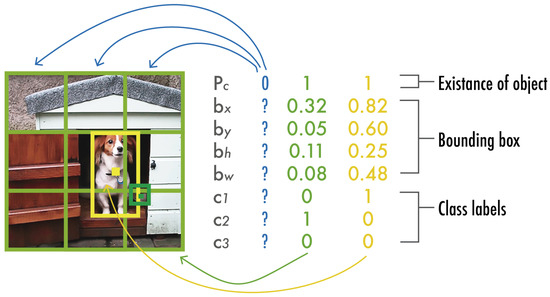
\includegraphics[width=\textwidth]{yolov1raster.jpg}
    \end{subfigure}
    \caption[YOLOv1 Raster] {Vereinfachte YOLOv1 Ausgabevorhersage bei einem 9x9 Raster mit 3 Klassen (blau, grün, gelb).
  Quelle: \cite{terven2023review}, Abb.~5, CC BY 3.0, ins Deutsche übertragen.}
    \label{fig:yolov1raster}
\end{figure}

\noindent Spätere Generationen wie YOLOv8 \cite{jocher2023yolov8} haben dieses Prinzip weiterentwickelt, unter anderem durch Vorhersagen auf mehreren Skalen und einen entkoppelten Head \cite{cheng2024yoloworld}. Es ist daher nicht unverändert auf moderne YOLO-Modelle übertragbar. Moderne YOLO-Netze lassen sich vereinfacht in drei Abschnitte gliedern \cite{cheng2024yoloworld} ()\cref{fig:backbone-neck-head}. Der Backbone extrahiert aus dem Eingabebild Features und überführt es schrittweise in eine kompakte Repräsentation. Der Neck führt diese Repräsentationen aus verschiedenen Ebenen zusammen und bereitet sie auf. Der Head berechnet daraus die finalen Bounding Boxes, Confidence Scores und Klassenwahrscheinlichkeiten. 

\begin{figure}[H]
  \centering
  \resizebox{\linewidth}{!}{\begin{tikzpicture}[node distance=7mm]
  \node[figbox] (in) {Eingabe-\\bild};
  \node[figbox, sblue, right=of in, minimum height=2.2cm, minimum width=1.1cm] (b1) {};
  \node[figbox, sblue, right=1mm of b1, minimum height=1.7cm, minimum width=0.9cm] (b2) {};
  \node[figbox, sblue, right=1mm of b2, minimum height=1.3cm, minimum width=0.7cm] (b3) {};
  \node[figbox, sblue, right=1mm of b3, minimum height=0.9cm, minimum width=0.5cm] (b4) {};
  \node[figbox, sorange, right=14mm of b4, minimum height=1.8cm, text width=2.2cm] (neck) {Neck\\[-1pt]{\footnotesize führt Merkmale zusammen}};
  \node[figbox, sgreen, right=of neck, minimum height=1.8cm, text width=2.6cm] (head) {Head\\[-1pt]{\footnotesize Bounding Boxes, Confidence Scores, Klassen}};
  \node[figbox, right=of head] (out) {Aus-\\gabe};
  \node[figlabel, above=2mm of b2.north east] {Backbone};
  \draw[figarrow] (in) -- (b1);
  \draw[figarrow] (b4) -- (neck);
  \draw[figarrow] (neck) -- (head);
  \draw[figarrow] (head) -- (out);
\end{tikzpicture}
}
  \caption[Aufbau eines YOLO-Netzwerks] {Vereinfachter Aufbau eines YOLO-Netzwerks aus Backbone, Neck und Head. Eigene Darstellung nach dem Aufbau aus \cite{cheng2024yoloworld}.}
  \label{fig:backbone-neck-head}
\end{figure}

\noindent Die in Backbone und Neck entstehenden Repräsentationen entsprechen den Features im Sinne von \cref{sec:merkmale}. Die in dieser Arbeit eingesetzten Modelle bauen auf YOLOv8 \cite{cheng2024yoloworld} auf (vgl. \cref{sec:modelle}).

%**********Merkmale im Kontext dieser Arbeit*************
\section{Merkmale im Kontext dieser Arbeit}
\label{sec:merkmale}
Der Begriff „Merkmal“, im Englischen „Feature“, wird je nach Fachgebiet unterschiedlich verwendet. Für die Detektion und den Vergleich von Münzbildern sind zwei Bedeutungen relevant, die im Folgenden voneinander abgegrenzt werden.
Im numismatischen Sprachgebrauch bezeichnet ein Merkmal ein für Menschen sichtbares und inhaltlich interpretierbares Element einer Münze, beispielsweise ein Herrscherporträt, eine Legende, ein Symbol oder eine Tierdarstellung (vgl. \cref{sec:glnumismatik}). Ein solches Merkmal lässt sich räumlich eingrenzen und einer Kategorie zuordnen. In diesem Sinne wird der Begriff in dieser Arbeit verwendet: Ein visuelles Merkmal ist ein abgrenzbarer Bildbestandteil, der von YOLO als Objekt lokalisiert und einer Klasse zugeordnet wird (vgl. \cref{sec:ooyolo}).
In der Bildverarbeitung und im maschinellen Lernen bezeichnet ein Feature dagegen eine numerische Eigenschaft der Eingabedaten, anhand derer ein Modell Bilddaten beschreibt und unterscheidet. Neuronale Netze erlernen solche Features während des Trainings selbstständig (vgl. \cref{sec:glmaschinelleslernen}). Mehrere Features werden zu einem Feature-Vektor 
$ A = (a_1, a_2, \dots, a_n) $ zusammengefasst, einer geordneten Folge von Werten \cite{duda2001pattern,bishop2006pattern} \todo{Bücher: Kapitel/Seiten nachschauen}. Die einzelnen Komponenten sind für Menschen in der Regel nicht interpretierbar \cite{montavon2018methods}. 
Für den Bildausschnitt eines detektierten Merkmals lässt sich ein Feature-Vektor aus einer internen Schicht des Netzwerks bestimmen \cite{ultralytics-predict,zhang2019recent}. Das Merkmal ist damit die für Menschen interpretierbare Ebene, der Feature-Vektor die numerische Repräsentation desselben Bildausschnitts. Die Extraktion wird in \cref{sec:vorgehen} beschrieben, die technische Umsetzung in \cref{sec:implementierung}.
Zwei Feature-Vektoren $ A $ und $ B $ gleicher Dimension $ n $ lassen sich mithilfe von Distanz- oder Ähnlichkeitsmaßen vergleichen. In dieser Arbeit werden drei gebräuchliche Maße verwendet:
\begin{itemize}
    \item Die Manhattan-Distanz summiert die Beträge der Differenzen \cite{aggarwal2001surprising}: \[ d_1(A, B) = \sum_{i=1}^{n}|a_i - b_i| \] Abweichungen gehen linear ein, einzelne große Komponenten dominieren das Ergebnis daher weniger.
    \item Die euklidische Distanz ist der geradlinige Abstand zweier Punkte im $n$-dimensionalen Raum \cite{wikipedia-euklidischer-abstand}: \[ d_2(A, B)= \sqrt{\sum_{i=1}^{n}(a_i - b_i)^2} \] Da die Differenzen quadriert werden, gehen einzelne große Abweichungen besonders stark in den Wert ein.
    \item Die Kosinus-Ähnlichkeit misst den Winkel zwischen zwei Vektoren \cite{manning2008introduction}: \[ \cos(A, B) = \frac{A \cdot B}{||A|| \cdot ||B||} \] Der Wert liegt zwischen $ -1 $ und $ 1 $. Er hängt nur von der Richtung der Vektoren ab, nicht von ihrer Länge.
    \todo{Buch: Abschnitt 6.3 bzw. Goodfellow nachschauen}
\end{itemize}
Bei den beiden Distanzen bedeutet ein kleiner Wert eine hohe Ähnlichkeit, bei der Kosinus-Ähnlichkeit ein großer. Die drei Maße gewichten Unterschiede zwischen Vektoren verschieden. Welches sich für den Vergleich von Merkmalen auf Münzbildern eignet, ist vorab nicht bekannt. Die Auswahl und Anwendung werden ebenfalls in \cref{sec:vorgehen} beschrieben.
%% !TeX root = ../Thesis.tex

%*****************************************
\chapter{Related Work}\label{ch:relatedwork}
%*****************************************
\glsresetall % Resets all acronyms to not used

\lipsum[44]
\lipsum[44]
\lipsum[44]
\lipsum[44]
\lipsum[44]
\lipsum[44]


\iftoggle{cts@parts}{
	\cleardoublepage % ensure that the PDF bookmark to the following part points to the right page
	%\ctparttext{Description of the second part.} % -- TemplateKnob (adjust or leave it)
	\part{Contributions}
}{}

% !TeX root = ../Thesis.tex

%************************************************
\chapter{Entwurf}\label{ch:entwurf}
%************************************************
\glsresetall % Resets all acronyms to not used

%****************Gesamtansatz und Datengrundlage****************************
\section{Gesamtansatz und Datengrundlage}
\label{sec:gesamtansatzdatengrundlage}
\textbf{Gesamtansatz}

\noindent Dieses Kapitel beschreibt den Ansatz zur Detektion und zum Vergleich visueller Merkmale auf antiken Münzbildern. Er besteht aus vier Schritten. Zunächst wird ein Münzbild eingelesen. Anschließend lokalisiert YOLO-World darauf einzelne visuelle Merkmale und ordnet sie einer Klasse zu, etwa Porträt, Symbol oder Inschrift. Für jedes detektierte Merkmal wird ein Feature-Vektor extrahiert (vgl. \cref{sec:merkmale}). Diese Vektoren werden mit den Vektoren der in einer Datenbank hinterlegten Münzen verglichen, und die ähnlichsten Münzen werden ausgegeben. Die Auswertung folgt in \cref{ch:evaluation}.

\begin{figure}[H]
  \centering
  \resizebox{\linewidth}{!}{\begin{tikzpicture}[node distance=6mm]
  \node[figbox, text width=1.8cm] (s1) {Münzbild};
  \node[figbox, sblue, text width=2.4cm, right=of s1] (s2) {Merkmals-\\detektion};
  \node[figbox, sorange, text width=2.4cm, right=of s2] (s3) {Feature-\\Vektoren};
  \node[figbox, sgreen, text width=2.4cm, right=of s3] (s4) {Vergleich der Merkmale};
  \node[figbox, right=of s4, text width=1.8cm] (res) {Ergebnis};
  \node[cylinder, shape border rotate=90, draw=black!70, fill=black!5, aspect=0.25, minimum height=1.2cm, minimum width=1.4cm, font=\footnotesize, align=center, below=7mm of s4] (db) {Datenbank};
  \node[figlabel, below=1mm of db] {bereits verarbeitete Münzen};
  \node[cylinder, shape border rotate=90, draw=black!70, fill=black!5, aspect=0.25, minimum height=1.2cm, minimum width=1.4cm, font=\footnotesize, align=center, below=7mm of s2] (yolo) {YOLO-World-Modell};
  \foreach \a/\b in {s1/s2,s2/s3,s3/s4,s4/res} \draw[figarrow] (\a) -- (\b);
  \draw[figarrow] (yolo) -- (s2);
  \draw[figarrow] (db) -- (s4);
\end{tikzpicture}
}
  \caption[Ablauf des Gesamtansatzes]{Gesamtansatz dieser Arbeit: Auf dem Münzbild werden Merkmale detektiert, zu jedem Merkmal wird ein Feature-Vektor bestimmt, und diese Vektoren werden mit den Vektoren bereits verarbeiteter Münzen in der Datenbank verglichen. Eigene Darstellung.}
  \label{fig:pipeline}
\end{figure}

\noindent Im Mittelpunkt stehen damit die einzelnen Merkmale und nicht die Münze als Ganzes. Die Klasse eines detektierten Merkmals dient dabei der Gruppierung, verglichen werden die zugehörigen Feature-Vektoren. Ob die Klasse inhaltlich zutrifft, ist für den Vergleich nicht ausschlaggebend (vgl. \cref{sec:zielsetzungundforschungsfragen}). Zusätzlich soll der Ansatz ohne technisches Vorwissen nutzbar sein, etwa für Forschende der Numismatik. Dazu kann ein eigenes Münzbild bereitgestellt und mit den gespeicherten Münzen verglichen werden. Das System bietet außerdem einen Vergleich ganzer Münzbilder auf Basis des Gesamtbild-Vektors an. Dieser ist nicht Gegenstand der Untersuchung und dient nur als ergänzende Funktion der Anwendung.

\vspace{\baselineskip}

\noindent \textbf{Datengrundlage}

\noindent Die Münzbilder stammen aus dem Corpus Nummorum (CN) \cite{corpusnummorum,peter2024corpus}, einem Online-Portal für antike Münzen, die in der archaischen Zeit bis unter römischer Herrschaft in den Regionen Thrakien, Moesia Inferior, Mysien und der Troas geprägt wurden. Die Datenbasis besteht aus Münzen des Münzkabinetts Berlin und aus Gipsabdrücken (engl. Plaster Casts) von Münzen, die an der Berlin-Brandenburgischen Akademie der Wissenschaften (BBAW) aufbewahrt werden und aus zahlreichen, heute teilweise nicht mehr vorhandenen Sammlungen stammen \cite{cn-about}. Daneben werden digitale Museumskataloge integriert, und Nutzer können eigene Münzen hochladen \cite{cn-about}. Das Portal umfasst rund 41.000 Münzen (Stand: 5.\ Oktober 2026)\cite{corpusnummorum}. Die Zahl wächst laufend. Davon werden 200 über die öffentliche API bezogen \cite{cn-data-api}, damit die Auswertung im Rahmen der Arbeit möglich bleibt. Die Bilder zeigen daher je nach Münze ein Original oder einen Gipsabdruck. Ein Gipsabguss
formt nur die Oberfläche der Münze ab, Farbe und Patina sind darauf daher nicht erkennbar. Abnutzung bleibt im Relief erkennbar, Korrosion nur, soweit sie die Oberfläche verändert hat. Die Abbildungen der Gipsabgüsse dürfen für wissenschaftliche Zwecke unter CC BY-NC-SA verwendet werden, für Aufnahmen der Originale liegen die Rechte bei den jeweiligen Rechteinhabern \cite{cn-bildrechte}.

Die Münzen wurden in aufsteigender ID-Reihenfolge abgerufen. Münzen ohne Vorderseitenbild oder ohne Stempel-ID wurden dabei übergangen. Eine Stempelgruppe wurde gebildet, sobald zehn Münzen mit demselben Vorderseitenstempel vorlagen; das wurde 20-mal wiederholt. Die Coin-IDs der 200 Münzen liegen zwischen 348 und 3561. Die Stempelzuordnung stammt aus der CN-Datenbank \cite{cn-about}. Die Gruppen dienen als Grundwahrheit für die Auswertung (vgl. \cref{ch:evaluation}). Alle 200 Münzen besitzen ein Vorderseitenbild, 199 ein Rückseitenbild. Insgesamt liegen 242 Vorderseiten- und 250 Rückseitenbilder vor; 51 Münzen haben auf mindestens einer Seite mehr als ein Bild. Die Zusammensetzung nach Bildart, Region, Münzstätte und Datierung zeigt \cref{tab:muenzdaten}, die einzelnen Stempelgruppen \cref{tab:stempelgruppen}.
Die Bilder werden als Vorschaubilder der Größe [Wert]\todo{Wert einfügen} geladen. Sie werden nicht weiterverarbeitet; lediglich das Modell skaliert sie intern auf die Eingabegröße [Wert]\todo{Wert einfügen}.
% Please add the following required packages to your document preamble:
% \usepackage[table,xcdraw]{xcolor}
% Beamer presentation requires \usepackage{colortbl} instead of \usepackage[table,xcdraw]{xcolor}
\begin{table}[H]
\centering
\begin{tabular}{|l|l|}
\hline
%\rowcolor[HTML]{EFEFEF} 
\textbf{Merkmal}                                & \textbf{Wert}                             \\ \hline
Münzen                                          & 200                                       \\ \hline
Stempelgruppen (obverse)                    & 20                                        \\ \hline
Münzen je Gruppe                                & 10                                        \\ \hline
Münzen mit Vorderseitenbild                     & 200                                       \\ \hline
Münzen mit Rückseitenbild                       & 199                                       \\ \hline
Bilder Vorderseite/Rückseite                    & 242/250                                   \\ \hline
Münzen mit \textgreater{1} Bild pro Seite & 51 (Vorderseite: 42, Rückseite: 51)                                        \\ \hline
Bildart                                         & [Foto: x, Gipsabdruck: y] \\ \hline
Regionen                                        & Thrakien: 190, ohne Angabe: 10                          \\ \hline
Münzstätten                                     & \makecell[l]{Byzantion: 110, Perinthos: 80, \\ Nikaia: 10}            \\ \hline
Datierung                                       & \makecell[l]{Ende 1./Mitte 2. Jh. - ca. 253--268 \\ n. Chr; 7 Münzen ohne Angabe}               \\ \hline
\end{tabular}
\caption{Überblick der verwendeten Münzdaten}
\label{tab:muenzdaten}
\end{table}

%****************Verwendete YOLO-Modelle****************************
\section{Verwendete YOLO-Modelle}
\label{sec:modelle}
In dieser Arbeit werden zwei YOLO-Modelle betrachtet. Den Ausgangspunkt bildete YOLOv8 \cite{jocher2023yolov8}, das in der vortrainierten Form ohne eigenes Nachtraining eingesetzt wurde. Untersucht werden sollte, ob ein nicht auf Münzen angepasstes Modell überhaupt Merkmale auf antiken Münzbildern detektiert. Das Modell wurde auf dem COCO-Datensatz \cite{lin2014microsoft} trainiert, der 80 Klassen alltäglicher Objekte umfasst \cite{ultralytics-yolov8}. Münzspezifische Merkmale wie Legenden oder Gottheiten sind darin nicht enthalten, die Ergebnisse waren entsprechend unbefriedigend (vgl. \cref{sec:ergebnisse}) \todo{oder appendix?}. YOLOv8 bleibt in der Anwendung nutzbar, steht aber nicht mehr im Zentrum der Forschungsfrage.

Die feste Klassenmenge war damit die zentrale Einschränkung. Ein wesentliches Kriterium für den weiteren Verlauf war daher, visuelle Merkmale mit möglichst geringem oder ohne aufgabenspezifisches Training detektieren zu können, ohne an vorgegebene Klassen gebunden zu sein. Dafür wurde YOLO-World \cite{cheng2024yoloworld} ausgewählt. Das Modell erkennt Objektklassen anhand von Textbeschreibungen im Zero-Shot-Verfahren (vgl. \cref{sec:glmaschinelleslernen}) \cite{cheng2024yoloworld,ultralytics-yoloworld}. CN stellt zwar einen Datensatz mit Motivklassen bereit, jedoch ohne Annotationen der Merkmalspositionen \cite{cn-object-detection-dataset}. Für antike Münzbilder relevante Merkmale können so untersucht werden, ohne zuvor einen annotierten Trainingsdatensatz zu erstellen. YOLO-World erweitert die in \cref{sec:ooyolo} beschriebene Detektion und baut auf der Architektur von YOLOv8 auf. Klassische YOLO-Modelle sind auf die Klassen beschränkt, die beim Training annotiert waren. YOLO-World ermöglicht dagegen die Detektion anhand frei formulierter Textbeschreibungen (Open Vocabulary). Dazu wird der Detektor mit dem vortrainierten Text-Encoder des CLIP-Modells \cite{radford2021learning} kombiniert. Dieser wandelt Texte in Vektoren um, die mit den vom Detektor erzeugten Objekt-Repräsentationen verglichen werden (vgl. \cref{sec:merkmale}) \cite{cheng2024yoloworld}. Im Netzwerk werden Bild- und Textinformationen im sogenannten RepVL-PAN, einer Erweiterung des Necks, verknüpft \cite{cheng2024yoloworld}.

\begin{figure}[H]
  \centering
  \resizebox{\linewidth}{!}{\begin{tikzpicture}[node distance=7mm]
  \node[figbox] (in) {Eingabe-\\bild};
  \node[figbox, sblue, right=of in, minimum height=1.6cm] (bb) {Backbone};
  \node[figbox, sorange, right=of bb, minimum height=1.6cm] (neck) {Neck\\[-1pt]{\footnotesize (mit RepVL-PAN)}};
  \node[figbox, sgreen, right=of neck, minimum height=1.6cm] (head) {Head};
  \node[figbox, right=of head] (out) {Boxen +\\Klassen};
  \draw[figarrow] (in) -- (bb);
  \draw[figarrow] (bb) -- (neck);
  \draw[figarrow] (neck) -- (head);
  \draw[figarrow] (head) -- (out);
  % Textzweig
  \node[figbox, spurple, above=1.4cm of in, xshift=-2mm] (pr) {Textbeschreibungen\\[-1pt]{\footnotesize (Prompts)}};
  \node[figbox, spurple, right=of pr] (clip) {CLIP-Text-\\Encoder};
  \node[figbox, spurple, right=of clip] (emb) {Text-\\Vektoren};
  \draw[figarrow, figpurple] (pr) -- (clip);
  \draw[figarrow, figpurple] (clip) -- (emb);
  \draw[figarrow, figpurple] (emb.south) -- (neck.north) node[midway, right, figlabel, align=left] {Verknüpfung mit\\Bildinformation};
\end{tikzpicture}
}
  \caption[Aufbau von YOLO-World]{Vereinfachter Aufbau von YOLO-World: Textbeschreibungen (Prompts) werden vom CLIP-Text-Encoder in Vektoren umgewandelt und im RepVL-PAN, einer Erweiterung des Necks, mit der Bildinformation verknüpft. Eigene Darstellung in Anlehnung an~\cite{cheng2024yoloworld}}
  \label{fig:yolo-world}
\end{figure}

Die Leistung eines Detektors hängt von der Architektur, den Trainingsdaten und dem Bildmaterial ab. Kleine, schlecht sichtbare oder teilweise verdeckte Objekte erschweren die Detektion, ebenso starke Unterschiede innerhalb einer Klasse oder schwer abgrenzbare Klassen \cite{liu2020deep}. Bei antiken Münzbildern treten auch Probleme auf wie Korrosion und Abnutzung (vgl. \cref{sec:glnumismatik}), die Motive und Legenden teilweise unkenntlich machen~\cite{cooper2020learning,anwar2026reading}.
Stempelunterschiede führen zu Abweichungen innerhalb derselben Motivklasse~\cite{wikipedia-muenzpraegung}. Zudem wurden im Rahmen der Recherche für diese Arbeit keine Untersuchungen gefunden, in denen YOLO-World auf Münzbildern trainiert oder angepasst wurde. YOLO-Varianten wurden dagegen bereits zur Zeichenerkennung auf Münzen eingesetzt~\cite{anwar2026reading}.

%****************Vorgehen****************************
\section{Vorgehen}
\label{sec:vorgehen}
Das Vorgehen besteht aus drei aufeinander aufbauenden Schritten: Merkmalsdetektion, Vektorextraktion und Vergleich.

\vspace{\baselineskip}

\noindent \textbf{Merkmalsdetektion}

\noindent Vorder- und Rückseite werden getrennt betrachtet, Eingabe ist jeweils das Bild einer Münzseite. YOLO-World sucht darauf nach einer festen Liste von 57 englischen Textbeschreibungen (Prompts), die sich an den typischen Motiven antiker Münzen aus \cref{sec:glnumismatik} orientiert (vollständige Liste in \cref{app:example}). \todo{Ergänzen: Wie ist die Liste entstanden, zum Beispiel aus den Beschreibungen der CN-Münzen, und wurde sie angepasst?} Eine Detektion gilt als gültig, wenn der Confidence Score 0,005 überschreitet. Der niedrige Wert wurde gewählt, weil bei höheren Schwellen kaum Detektionen entstanden, wie in den nachfolgenden \cref{tab:schwellenwerte_rückseite,tab:schwellenwerte_vorderseite} zu sehen ist. 

\begin{table}[H]
\centering
\caption{Detektionen auf Rückseitenbildern bei verschiedenen Schwellenwerten (250 Bilder)}
\label{tab:schwellenwerte_rückseite}
\begin{tabular}{|l|r|r|r|r|}
\hline
\textbf{Schwellenwert}         & 0{,}005 & 0{,}01 & 0{,}05 & 0{,}5  \\ \hline
\textbf{Detektionen}           & 974     & 552    & 293    & 3      \\ \hline
\textbf{Ø Detektionen je Bild}             & 3{,}90  & 2{,}21 & 1{,}17 & 0{,}01 \\ \hline
\textbf{Bilder ohne Detektion} & 15      & 21     & 43     & 247    \\ \hline
\textbf{Klassen}               & 22      & 13     & 11      & 2      \\ \hline
\end{tabular}
\end{table}

\begin{table}[H]
\centering
\caption{Detektionen auf Vorderseitenbildern bei verschiedenen Schwellenwerten (242 Bilder)}
\label{tab:schwellenwerte_vorderseite}
\begin{tabular}{|l|r|r|r|r|}
\hline
\textbf{Schwellenwert}         & 0{,}005 & 0{,}01 & 0{,}05 & 0{,}5  \\ \hline
\textbf{Detektionen}           & 905     & 543    & 312    & 7      \\ \hline
\textbf{Ø Detektionen je Bild}             & 3{,}74  & 2{,}24 & 1{,}29 & 0{,}03 \\ \hline
\textbf{Bilder ohne Detektion} & 12      & 16     & 41     & 235    \\ \hline
\textbf{Klassen}               & 23      & 18     & 9      & 2      \\ \hline
\end{tabular}
\end{table}

Überlappende Detektionen werden durch die Standard-NMS von Ultralytics zusammengefasst (Parameter in \cref{app:example}). Detektionen, deren Bounding Box mindestens 85\,\% der Bildfläche einnimmt, werden verworfen, damit nicht das gesamte Münzbild als Merkmal gilt (Parameter \texttt{max\_area\_ratio}, \cref{app:example}). \todo{Begründung für 0,85 ergänzen} Eine weitere Nachbearbeitung findet nicht statt. Pro Detektion werden Klasse, Confidence Score und die auf die Bildgröße normierte Bounding Box gespeichert.

\vspace{\baselineskip}

\noindent \textbf{Vektorextraktion}

\noindent Zu jeder Detektion wird ein Feature-Vektor bestimmt. Dazu wird die Bounding Box aus dem Originalbild ausgeschnitten und erneut durch YOLO-World geleitet. Als Vektor dient die Ausgabe des letzten Neck-Blocks (Schicht 21), die über die räumlichen Dimensionen gemittelt wird (Dimension [512]). Der Vektor beschreibt damit den Ausschnitt ohne Kontext des Gesamtbildes. Ebenso wird für jedes Münzbild ein Gesamtbild-Vektor erzeugt. Alle Vektoren werden mit Klasse, Confidence Score, Bounding Box und Münzseite in der Datenbank gespeichert.

\vspace{\baselineskip}

\noindent \textbf{Vergleich}

\noindent Verglichen werden Feature-Vektoren einzelner Merkmale. Der Nutzer wählt ein detektiertes Merkmal und eine Münzseite aus. Das Merkmal wird nur mit Merkmalen derselben Klasse auf derselben Münzseite verglichen \todo{Umgang mit verwandten Klassen ergänzen}. Zusätzlich müssen Position und Größe ähnlich sein. Der Abstand der Boxmittelpunkte darf 0,15 (normierte Koordinaten) nicht überschreiten, und das Flächenverhältnis der Boxen muss mindestens 0,5 betragen.
Für zwei Vektoren A und B der Dimension n werden die drei Maße aus \cref{sec:merkmale} verwendet. 
Die beiden Distanzen $d$ (euklidisch, Manhattan) werden über $s = \frac{1}{1+d}$ in eine Ähnlichkeit $s \in (0, 1]$ umgerechnet, die Kosinus-Ähnlichkeit wird unverändert verwendet ($s \in [-1, 1]$). Die Umrechnung der Distanzen ist monoton und ändert das Ranking nicht. Die Ähnlichkeitswerte verschiedener Maße sind wegen der unterschiedlichen Wertebereiche nicht direkt vergleichbar, verglichen werden die Rangfolgen. Die Maße erfassen unterschiedliche Aspekte der Ähnlichkeit. Da vorab nicht bekannt ist, welches sich am besten eignet, werden alle drei parallel eingesetzt und in \cref{ch:evaluation} verglichen. 
Pro Münze zählt der höchste Ähnlichkeitswert über alle passenden Merkmale. Die Münzen werden nach Ähnlichkeit absteigend sortiert, und die ähnlichsten [1 bis 5] werden ausgegeben. 


%****************Bewertungskonzept****************************
\section{Bewertungskonzept}
\label{sec:bewertungskonzept}
Ob sich Münzen desselben Stempels anhand einzelner Merkmale wiederfinden lassen, wird mithilfe der Stempelgruppen als Grundwahrheit untersucht (vgl. \cref{sec:gesamtansatzdatengrundlage}). Für jede Münze wird geprüft, ob Münzen derselben Gruppe unter den ähnlichsten Treffern liegen. Verglichen werden die Merkmalsklassen und die drei Ähnlichkeitsmaße. Ergänzend werden einzelne Fälle qualitativ untersucht. Das genaue Vorgehen und die Kennzahlen werden in \cref{sec:evaluationsaufbau} beschrieben.
% !TeX root = ../Thesis.tex

%************************************************
\chapter{Umsetzung}\label{ch:umsetzung}
%************************************************
\glsresetall % Resets all acronyms to not used
Dieses Kapitel beschreibt die Umsetzung des in \cref{ch:entwurf} entwickelten Ansatzes. \cref{sec:rahmenbedingungen} nennt die technischen Rahmenbedingungen, \cref{sec:implementierung} die Implementierung der einzelnen Komponenten und \cref{sec:herausforderungen} die Herausforderungen bei der Umsetzung.

%**********Technische Rahmenbedingungen*************
\section{Technische Rahmenbedingungen}
\label{sec:rahmenbedingungen}
Die Anwendung wurde in Python [Version] \todo{Wert einfügen} entwickelt und lokal auf [CPU/GPU, Modell, Arbeitsspeicher] \todo{Wert einfügen} unter [Betriebssystem] \todo{Wert einfügen} betrieben. Tabelle \cref{tab:bibliotheken} zeigt die eingesetzten Bibliotheken.

\begin{table}[htbp]
    \centering
    \small
    \begin{tabularx}{\textwidth}{|l|l|X|}
        \hline
        \textbf{Bibliothek} & \textbf{Version} & \textbf{Zweck} \\
        \hline
        Ultralytics &  & Detektion mit YOLO-World, Extraktion der Feature-Vektoren \\
        \hline
        OpenCV &  & Dekodieren der Bilder \\
        \hline
        Requests &  & Abruf der Daten über die CN-Schnittstelle \\
        \hline
        FastAPI, Uvicorn &  & Backend, lokale Bereitstellung \\
        \hline
        SQLite &  & Speicherung der Münzdaten und Vektoren \\
        \hline
    \end{tabularx}
    \caption{Verwendete Bibliotheken}
    \label{tab:bibliotheken}
\end{table}

\noindent Als Modell dient YOLOv8s-World-v2 (vgl. \cref{sec:modelle}). Die Benutzeroberfläche besteht aus HTML, CSS und JavaScript.Parameter wie Modellpfade, Prompt-Liste, Schwellenwert, Batchgröße und die Werte des Positions- und Größenfilters stehen in separaten JSON-Konfigurationsdateien und lassen sich ohne Änderung des Programmcodes anpassen. Die verwendeten Werte sind in Anhang B zusammengestellt.

%**********Implementierung*************
\section{Implementierung}
\label{sec:implementierung}
\textbf{Aufbau}

\noindent Die Anwendung ist modular aufgebaut. Der \lstinline|Request_Handler| bezieht Daten und Bilder aus der CN-Schnittstelle, der \lstinline|DatabaseHandler| übernimmt die Datenbank, der \lstinline|YoloHandler| die Detektion und Vektorextraktion, der \lstinline|CoinMatcher| mit dem \lstinline|VectorComparator| die Suche, und der \lstinline|ApiHandler| verbindet diese Komponenten mit der Oberfläche (vgl. Abbildung \cref{app:example} \todo{UML einfügen}).

\vspace{\baselineskip}

\noindent \textbf{Datenbeschaffung und Speicherung}

\noindent Der \lstinline|Request_handler| ruft Metadaten und Bild-URLs ab und lädt die Bilder, die mit OpenCV als NumPy-Arrays dekodiert werden. Vorder- und Rückseite werden getrennt behandelt, pro Seite können mehrere Bilder vorliegen. Die Datenbank wird gruppenweise aufgebaut: Sobald zehn Münzen mit demselben Vorderseitenstempel vorliegen, werden ihre Bilder verarbeitet und die Münzen gespeichert. Die Münzen liegen in einer SQLite-Tabelle. Metadaten stehen in eigenen Spalten, Bild-URLs, Literatur und die erzeugten Merkmalsinformationen als JSON-Text. Letztere sind nach Münzseite und Bild gegliedert. Pro Bild gibt es den Gesamtbild-Vektor und je Klasse eine Liste von Detektionen mit Confidence Score, normierter Bounding Box und Feature-Vektor.

\vspace{\baselineskip}

\noindent \textbf{Detektion und Vektorextraktion}

\noindent Der \lstinline|YoloHandler| lädt Modell und Einstellungen aus der Konfigurationsdatei und setzt die Prompt-Liste beim Anlegen einmalig. Für die Detektion wird das Modell mit dem konfigurierten Schwellenwert aufgerufen (Anhang B). Gespeichert werden Klasse, Confidence Score und die auf die Bildgröße normierte Bounding Box. Anschließend wird jede Box aus dem Originalbild ausgeschnitten. Die Feature-Vektoren entstehen über den Parameter \lstinline|embed| der Ultralytics-Vorhersage, der die Ausgabe ausgewählter Schichten liefert. Verwendet wird Schicht 21, der letzte Block des Necks (C2fAttn, P5/32), dessen Ausgabe an den Detektionskopf weitergegeben wird \todo{QUELLE: yolov8-worldv2.yaml}. Die Ausgabe wird räumlich gemittelt \todo{QUELLE: Ultralytics, tasks.py} und ergibt einen Vektor der Dimension 512 \todo{Wert prüfen}. Der Durchlauf endet an dieser Schicht, der Detektionskopf wird nicht ausgeführt. Vektoren entstehen für das Gesamtbild und für jeden Ausschnitt. Die Ausschnitte werden in Batches zu je 16 Bildern verarbeitet, die Größe ist konfigurierbar.

\vspace{\baselineskip}

\noindent \textbf{Vergleich}

\noindent Der \lstinline|CoinMatcher| lädt beim Start alle Münzen mit ihren Vektoren in den Arbeitsspeicher und vergleicht eine Anfrage sequenziell mit allen. Der \lstinline|VectorComparator| setzt die Maße aus \cref{sec:merkmale} um und rechnet sie in eine Ähnlichkeit zwischen 0 und 1 um. Die Kosinus-Ähnlichkeit wird dazu linear von $ [-1, 1] $ auf $ [0, 1] $ abgebildet, die beiden Distanzen $ d $ als $ \frac{1}{1+d} $. Beim objektbasierten Vergleich wählt die nutzende Person ein detektiertes Merkmal aus. Dessen Ausschnitt wird durch das Modell geführt, der Vektor wird  mit den Vektoren gleicher Klasse auf der gewählten Münzseite verglichen. Treffer müssen den Positions- und Größenfilter erfüllen (Werte in \cref{app:example}); beide Werte sind konfigurierbar. Pro Münze zählt de rhöchste Wert, danach werden die münzen absteigend sortiert und die ersten \lstinline|top_k| zurückgegeben. Ähnliche Klassen werden nicht zusammengefasst.

Zusätzlich ist ein Gesamtbildvergleich umgesetzt, bei dem der Vektor des Gesamtbildes mit denen in der Datenbank verglichen wird. Hat eine Münze mehrere Bilder einer Seite, zählt das ähnlichste. Er ergänzt die Anwendung und ist nicht Gegenstand der Untersuchung (vgl. \cref{sec:gesamtansatzdatengrundlage}).

\vspace{\baselineskip}

\noindent \textbf{Backend und Oberfläche}

\noindent Das Backend stellt fünf Routen bereit: 
\begin{itemize}
    \item zwei zum Abruf von Münzen,
    \item \lstinline|/api/search/detect| für die Detektion,
    \item \lstinline|/api/search/object| für den objektbasierten Vergleich und
    \item \lstinline|/api/search/vector| für den Gesamtbildvergleich.
\end{itemize}
Die Oberfläche läuft in zwei Schritten. Der Nutzer lädt ein Münzbild hoch, bei aktivierter Detektion erscheinen die Bounding Boxes mit Klasse und Confidence Score, und eines der Merkmale wird per Klick oder Dropdown gewählt. Anschließend werden Münzseite, Anzahl der Ergebnisse (1 bis 5) und Ähnlichkeitsmaß eingestellt und die Suche gestartet. Die Ergebnisse erscheinen mit Bild, Ähnlichkeitswert, Münzinformationen und Suchzeit.

%**********Herausforderungen*************
\section{Herausforderungen}
\label{sec:herausforderungen}
\textbf{Vektoren für einzelne Merkmale}

\noindent Die Embedding-Funktion von Ultralytics liefert einen Vektor pro Bild, nicht pro Bounding Box. Um Vektoren einzelner Merkmale zu erhalten, werden die Boxen ausgeschnitten und einzeln durch das Modell geführt \todo{bestätigen: Grund für den Ausschnitt statt eines Pooling-Verfahrens auf der Feature-Karte}. Das hat zwei Folgen; der Vektor beschreibt das Merkmal ohne Kontext des Gesamtbildes und jede Detektion kostet einen zusätzlichen Modellaufruf.

\vspace{\baselineskip}

\noindent \textbf{Abhängigkeit von der Prompt-Liste}

\noindent Die Schicht 21 bezieht die Textrepräsentationen der Prompts ein. Die Vektoren hängen daher von der Prompt-Liste ab. Anfrage und Datenbank müssen dieselbe Liste verwenden und bei jeder Änderung muss die Datenbank neu aufgebaut werden. Die Liste wird deshalb nur einmal in der Konfiguration festgelegt (\cref{app:example}).

\vspace{\baselineskip}

\noindent \textbf{Laufzeit beim Aufbau der Datenbank}

\noindent Der Aufbau erfordert viele Modellaufrufe. Je Bild einen für die Detektion und einen für den Gesamtbild-Vektor, dazu einen je detektiertem Ausschnitt. Wegen des niedrigen Schwellenwerts (vgl. \cref{sec:vorgehen}) entstehen pro Bild viele Detektionen, für die 200 Münzen insgesamt [Anzahl] \todo{Wert eintragen} Ausschnitte. \todo{Beschreibung des Problems: Bei einzelner Verarbeitung der Ausschnitte dauerte der Aufbau [Zeit], bei gleichzeitiger Übergabe [Problem].} Deshalb werden Bilder und Detektionen gruppenweise je Stempelgruppe verarbeitet und die Ausschnitte in Batches zu 16 Bildern an das Modell übergeben. Dadurch verkürzte sich der Aufbau auf [Zeit] \todo{Wert eintragen}. Die Suche selbst vergleicht die Anfrage sequenziell mit allen gespeicherten Vektoren und benötigt bei 200 Münzen [Messwert] \todo{Wert eintragen} Sekunden. Bei größeren Beständen wäre eine Vektorisierung oder ein Suchindex nötig.

\vspace{\baselineskip}

\noindent \textbf{Uneinheitliche Datenlage}

\noindent Pro Münzseite liegen null bis zwei Bilder vor, acht Münzen haben kein Vorderseitenbild. Die Datenstruktur ordnet Merkmale deshalb Münze, Seite und Bild zu, Münzen ohne Bild werden übersprungen, und pro Münze zählt das ähnlichste Bild.

% !TeX root = ../Thesis.tex

%************************************************
\chapter{Evaluation}\label{ch:evaluation}
%************************************************
\glsresetall % Resets all acronyms to not used

%*************Evaluationsaufbau***************
\section{Evaluationsaufbau}
\label{sec:evaluationsaufbau}
\noindent \textbf{Grundwahrheit/Ground Truth}

Als Grundwahrheit dienen die 20 Stempelgruppen mit je zehn Münzen (vgl. \cref{sec:gesamtansatzdatengrundlage}). Münzen derselben Gruppe weisen denselben Vorderseitenstempel auf und sollten sich daher besonders ähnlich sein (vgl. \cref{sec:glnumismatik}). Da die Gruppen anhand der Vorderseiten-ID gebildet wurden, wird die Auswertung auf den Vorderseiten durchgeführt. Für die Rückseiten gilt die Grundwahrheit nur eingeschränkt, da Münten mit gleichen Vorderseitenstempel unterschiedliche Rückseitenstempel haben können.

\vspace{\baselineskip}

\noindent \textbf{Protokoll}

\noindent Jede der 192 Münzen mit Vorderseitenbild dient als Anfrage und wird mit den übrigen 191 verglichen. Als Treffer gelten die 6 bis 9 anderen Münzen derselben Gruppe, die ein Vorderseitenbild besitzen. Für jede Klasse wird das Merkmal mit der höchsten Confidence der Anfrage-Münze verwendet \todo{Entscheidung bestätigen}. Es wird mit den Merkmalen derselben Klasse auf der Vorderseite der übrigen Münzen verglichen (vgl. \cref{sec:vorgehen}). Der Wert einer Münze ist die höchste Ähnlichkeit über alle ihre passenden Merkmale. Anfragen, auf denen die Klasse nicht detektiert wurde, gehen nicht in die Wertung dieser Klasse ein. Für jede Klasse wird daher angegeben, auf wie vielen Münzen sie vorkommt (n). Zusätzlich wird ein Gesamtwert gebildet, indem die Ähnlichkeiten über alle Klassen gemittelt werden, die bei Anfrage und Kandidat vorliegen \todo{Entscheidung bestätigen}.

\vspace{\baselineskip}

\noindent \textbf{Kennzahlen}

\noindent Bewertet wird die Reihenfolge der Suchergebnisse. Die Kennzahlen beziehen sich auf die ersten $k$ Münzen dieser Reihenfolge, also auf die Ergebnisse, die die Anwendung anzeigt. Da die Anwendung bis zu fünf Ergebnisse ausgibt, werden $k = 1$ und $k = 5$ betrachtet. HitRate@1 gibt den Anteil der Anfragen an, bei denen die ähnlichste Münze denselben Vorderseitenstempel hat. HitRate@5 gibt den Anteil der Anfragen an, bei denen mindestens eine der ersten fünf Münzen denselben Stempel hat. Beide Werte zeigen, wie oft eine Suche überhaupt zu einem Treffer führt. Precision@5 ist der Anteil der Treffer unter den ersten fünf Münzen, gemittelt über alle Anfragen. Sie zeigt, wie viele der angezeigten Ergebnisse im Durchschnitt passen. \todo{Quelle} Alle Werte werden pro Klasse und als Gesamtwert für jedes der drei Ähnlichkeitsmaße angegeben. Als Untergrenze dient der Wert, der sich bei einer zufälligen Reihenfolge ergibt. Er liegt für HitRate@1 und Precision@5 bei etwa [x]\,\% und für HitRate@5 bei etwa [y]\,\% \todo{Werte eintragen}.

\vspace{\baselineskip}

\noindent \textbf{Einflussfaktoren}

\noindent Zusätzlich werden die Ergebnisse nach Bildtyp (Fotos, Plaster Casts) getrennt ausgewertet, da diese sich in Darstellung und Kontrast unterscheiden. \todo{Optional: Ergebnisse mit und ohne Positions- und Größenfilter}

\vspace{\baselineskip}

\noindent \textbf{Einschränkungen}

\noindent Die Grundwahrheit gilt nur für Vorderseiten. Mit 200 Münzen sind die Ergebnisse als Tendenzen zu verstehen. Die Münzen wurden nicht zufällig, sondern in aufsteigender ID-Reihenfolge ausgewählt (vgl. \cref{sec:gesamtansatzdatengrundlage}). Der Zustand der Münzen und die Qualität der Bilder können die Ähnlichkeit beeinflussen, unabhängig vom Stempel (vgl. \cref{sec:glnumismatik}).

\vspace{\baselineskip}

\noindent \textbf{Testfälle}

%**************Ergebnisse********************
\section{Ergebnisse}
\label{sec:ergebnisse}
\textbf{Merkmalsdetektion}

\todo{daten aus tabellen nur obverse}

\vspace{\baselineskip}

\noindent \textbf{Vergleich}

\section{Qualitative Analyse}
\label{sec:qualitativeanalyse}
Die Kennzahlen zeigen, bei welchen Münzen der Ansatz funktioniert, aber nicht warum. Dazu werden 20 zufällig gewählte Münzen (fester Startwert) einzeln untersucht und anschließend einzelne Positiv- und Negativbeispiele getrennt davon gezeigt. Beschrieben werden Erhaltungszustand (dreistufige Skala \todo{Kriterien definieren}), Licht und Kontrast, Bildtyp und Klasse des Merkmals. Bei Fehlschlägen wird zunächst geprüft, ob die Bounding Box das Merkmal trifft. So lässt sich zwischen Fehlern der Detektion und Fehlern des Vergleichs unterscheiden. Die Analyse zeigt Zusammenhänge auf und keine Ursachen, da das Modell seine Entscheidungen nicht erklärt.

\iftoggle{cts@parts}{
	\cleardoublepage % ensure that the PDF bookmark to the following part points to the right page
	%\ctparttext{Description of the third part.} % -- TemplateKnob (adjust or leave it)
	\part{Discussion and Conclusion}
}{}

% !TeX root = ../Thesis.tex

%************************************************
\chapter{Diskussion}\label{ch:discussion} % $\mathbb{ZNR}$
%************************************************
\glsresetall % Resets all acronyms to not used

%************Beantwortung der Forschungsfragen**************
\section{Beantwortung der Forschungsfragen}
\label{sec:beantwortungfragen}
\begin{enumerate}
    \item \noindent Welche Grenzen zeigt ein Ansatz ohne münzspezifisches Training bei der Anwendung auf antike Münzbilder?

    \noindent Der Ansatz stößt an mehreren Stellen an Grenzen. Erstens liefert YOLO-World nur 23 (vorderseite) bzw. 22 (Rückseite) der 57 Prompts als Klasse mit meist niedriger Confidence (vgl. \cref{sec:ergebnisse}), und ob eine Klasse inhaltlich zutrifft, lässt sich ohne eigene Prüfung nicht sagen \todo{an qualitative Analyse anpassen}. Zweitens hängen Detektion und Vektoren von der festgelegten Prompt-Liste ab. Drittens [Einfluss von Erhaltungszustand und Bildtyp, aus Ergebnissen]. Viertens beschreibt ein Vektor das Merkmal ohne Kontext des Gesamtbildes. Zudem wird auf Münzen desselben Stempels häufig eine andere Klasse am sichersten detektiert, sodass nur 36\,\% der stempelgleichen Paare überhaupt verglichen werden (vgl. \cref{sec:ergebnisse}) Die Einzelheiten und die Grenzen der Untersuchung selbst behandelt \cref{sec:grenzen-untersuchung}.

\end{enumerate}

%*********Einordnung in bestehende Arbeiten**********************
\section{Einordnung in bestehende Arbeiten}
\label{sec:bestehendearbeiten}
Bildbasierte Verfahren für antike Münzen lassen sich nach ihrer Aufgabe in drei Gruppen einteilen. Die Arbeit liegt an der Schnittstelle dieser Gruppen, unterscheidet sich aber in einem Punkt von allen; sie verzichtet auf münzspezifisches Training.

\vspace{\baselineskip}

\noindent \textbf{Zuordnung ganzer Münzen} 

\noindent Guo et al. \cite{guo2023siamese} ordnen Münzbilder über ein Siamese-Netz mit Vision Transformern einer Prägung (Issue) zu, indem sie paarweise entscheiden, ob zwei Bilder zur selben Prägung gehören. Neue Prägungen lassen sich so ohne Neutraining ergänzen. Das Netz wird aber auf Münzpaaren trainiert, und verglichen wird die ganze Münze. Fare und Arandjelović \cite{fare2017ancient} untersuchen die Münzsuche systematisch im Hinblick auf den Erhaltungsgrad und nennen diesen eine zentrale Schwierigkeit. Der Erhaltungszustand spielt auch in dieser Arbeit eine Rolle (vgl. \cref{sec:qualitativeanalyse}).

\vspace{\baselineskip}

\noindent \textbf{Erkennung einzelner Motive und Zeichen} 

\noindent Cooper und Arandjelović \cite{cooper2020learning} trainieren je Motiv (z.\,B. Pferd, Adler, Schild) ein CNN, das erkennt, ob es auf der Rückseite vorkommt. Die Trainingslabels stammen aus Beschreibungstexten von Händlern, es wurden also keine Bildpositionen annotiert. Kim und Pavlovic \cite{kim2016discovering} suchen mit CNNs charakteristische Bildregionen je Münzklasse. Anwar \cite{anwar2026reading} behandelt einzelne Buchstaben als Objekte und trainiert verschiedene YOLO-Modelle nach, auf einem eigens annotierten Datensatz mit 38,808 Bounding Boxes. Das ist die engste Verbindung zu dieser Arbeit, denn auch dort wird ein YOLO-Detektor auf Münzbilder angewendet. Der Unterschied liegt darin, dass das Modell dort mit manuellen Annotationen nachtrainiert wird, hier jedoch ohne Nachtraining anhand von Textbeschreibungen detektiert. \todo{prüfen: 81\%, 84\%, NMI 0.959, 38.808 Boxen} \todo{anwar widerspruch: text 914\% und tabelle 90,4\%}

\vspace{\baselineskip}

\noindent \textbf{Stempelanalyse} 

\noindent Heinecke et al. \cite{heinecke2021unsupervised} gruppieren Münzbilder ohne Trainingsdaten nach dem Stempel, indem sie Schlüsselpunkte auf dem gesamten Münzbild vergleichen und die Gruppen statistisch bestimmen. Sie arbeiten auf Denaren aus der Zeit Neros und prüfen manuell, wie gut die Gruppen den echten Stempeln entsprechen. Das Ziel entspricht dem hier verwendeten Ansatz, Münzen desselben Stempels zu finden. Anders als hier werden aber keine einzelnen Merkmale detektiert und keine gelernten Feature-Vektoren verglichen.

\vspace{\baselineskip}

\noindent \textbf{Abgrenzung} 
\noindent Damit unterscheidet sich diese Arbeit in drei Punkten: Erstens kommt sie ohne Training und ohne Annotationen der Merkmalspositionen aus, wogegen die Verfahren zur Zuordnung und Motiverkennung \cite{guo2023siamese,cooper2020learning,anwar2026reading} auf münzspezifischen Daten trainiert werden. Zweitens wird nicht die ganze Münze verglichen, sondern einzelne lokalisierte Merkmale. Drittens dienen die Stempelgruppen aus dem Corpus Nummorum als Grundwahrheit für die Auswertung (vgl. \cref{sec:evaluationsaufbau}). Dafür wird auch weniger geleistet: Es werden nur 23 Klassen detektiert, die Stempelsuche wird auf 200 Münzen gezeigt, und eine inhaltliche Prüfung der Klassen fehlt \todo{an Ergebnisse anpassen}.

\vspace{\baselineskip}

\noindent \textbf{Vergleichbarkeit der Ergebnisse} 
\noindent Die Zahlen der genannten Arbeiten lassen sich nicht direkt mit den Ergebnissen dieser Arbeit vergleichen, da Aufgabe, Daten und Kennzahlen verschieden sind. Guo et al. berichten eine Genauigkeit von 81\,\% für die Zuordnung zu einer Prägung, Cooper und Arandjelović bis zu 84\,\% je Motiv, Anwar einen mAP50 von rund 90\,\% für Buchstaben. Heinecke et al. geben ein Clustermaß (NMI) von etwa 0,96 für Vorderseiten an. Diese Werte messen jeweils, ob etwas richtig eingeordnet wird. Hier wird gemessen, ob Münzen desselben Stempels unter den ähnlichsten Treffern liegen (HitRate@$k$, vgl. \cref{sec:evaluationsaufbau}). Die Ergebnisse dieser Arbeit liegen bei 17\,3\% (HitRate@1) und 46\,2\% (HitRate@5) \todo{aus \cref{sec:ergebnisse} einsetzen} und sind mit 200 Münzen als Tendenz zu verstehen. Ob ein Ansatz ohne Training den trainierten Verfahren nahekommt, lässt sich daraus nur eingeschränkt beantworten; ein Vergleich auf denselben Daten steht aus \todo{Formulierung nach den Ergebnissen anpassen}.

%***************Grenzen*****************************
\section{Grenzen}
\label{sec:grenzen}
\subsection{Grenzen des Ansatzes}
\label{sec:grenzen-ansatz}
\textbf{Bildmaterial} 

\noindent Die Bilder stammen teils von Originalen und teils von Gipsabgüssen und unterscheiden sich in Kontrast, Licht und Aufnahmebedingungen (vgl. \cref{sec:glnumismatik}). Zusammen mit Abnutzung und Korrosion kann dies die Ähnlichkeit zweier Münzen beeinflussen, unabhängig davon, ob sie vom selben Stempel stammen. Die Auswertung nach Bildtyp zeigt Unterschiede \todo{Ergebnis einsetzen}, trennt aber nicht von den Einflüssen des Erhaltungszustands.

\vspace{\baselineskip}

\noindent \textbf{Modell und Prompts} 

\noindent Die detektierten Klassen hängen von der Prompt-Liste mit 57 englischen Textbeschreibungen ab, die zu Beginn der Arbeit erstellt und nicht an die Motivbeschreibungen von CN angepasst wurde (vgl. \cref{sec:vorgehen}). Zudem hängen die Vektoren selbst von dieser Liste ab (vgl. \cref{sec:herausforderungen}), sodass ein anderes Vokabular zu anderen Ergebnissen führen kann. Ob eine detektierte Klasse inhaltlich zutrifft, wurde nur in der qualitativen Analyse an Stichproben geprüft (vgl. \cref{sec:qualitativeanalyse}). Der niedrige Schwellenwert von 0,005 führt zu vielen Detektionen mit geringer Confidence (vgl. \cref{sec:ergebnisse}). Auch der Grenzwert von 85\,\% der Bildfläche, ab dem Detektionen verworfen werden, wurde nicht systematisch bestimmt (vgl. \cref{sec:vorgehen}). 

Neben Yolov8s-World-v2 wurde Yolov8n verglichen, das auf der Vorderseite leicht bessere Trefferraten erzielt (vgl. \cref{tab:modelle_vorderseite,tab:modelle_rueckseite}). Die Unterschiede betragen fünf bis sieben von 200 Anfragen und sind daher gering. Der Modellvergleich beruht ausschließlich auf der Kosinus-Ähnlichkeit. Ob sich das Verhältnis der beiden Modelle mit der Manhattan-Distanz ändert, wurde nicht untersucht. \todo{falls doch, einfügen!}

\vspace{\baselineskip}

\noindent \textbf{Vektoren einzelner Merkmale} 

\noindent Der Vektor eines Merkmals wird aus dem ausgeschnittenen Bildausschnitt bestimmt und kennt den Kontext des Gesamtbildes nicht (vgl. \cref{sec:herausforderungen}). Ob Vektoren aus dem ganzen Bild mit Pooling auf der Feature-Karte bessere Ergebnisse liefern, wurde nicht untersucht.

\vspace{\baselineskip}

\noindent \textbf{Vergleich nur innerhalb einer Klasse} 

\noindent Merkmale werden nur mit Merkmalen derselben Klasse verglichen (vgl. \cref{sec:vorgehen}). Ob verwandte Klassen, die dasselbe Motiv unterschiedlich benennen, gemeinsam verglichen werden können, wurde im Rahmen dieser Arbeit nicht untersucht. Dadurch können Münzen desselben Stempels unverglichen bleiben, wenn auf ihnen verschiedene Klassen detektiert werden.

\subsection{Grenzen der Untersuchung}
\label{sec:grenzen-untersuchung}
\textbf{Umfang und Auswahl der Daten} 

\noindent Die Auswertung beruht auf 200 Münzen in 20 Stempelgruppen mit je zehn Münzen, die in aufsteigender ID-Reihenfolge und nicht zufällig aus dem Corpus Nummorum gewählt wurden (vgl. \cref{sec:gesamtansatzdatengrundlage}). Die Ergebnisse gelten daher für diese Auswahl und lassen sich nicht ohne Weiteres auf andere Prägungen, Epochen oder Regionen übertragen. Wegen der kleinen Gruppen könnten einzelne Münzen die Kennzahlen deutlich verändern.

\vspace{\baselineskip}

\noindent \textbf{Grundwahrheit} 

\noindent Als Grundwahrheit dienen die Stempelgruppen aus der CN-Datenbank \cite{cn-about}. Sie gilt nur für die Vorderseiten (vgl. \cref{sec:evaluationsaufbau}). Für die Rückseiten gibt es nur wenige Münzen mit gleichem Stempel, sie werden daher nur ergänzend ausgewertet. Die Güte der Auswertung hängt davon ab, dass die Zuordnung in CN korrekt ist. Sie wurde in dieser Arbeit nicht überprüft.

\vspace{\baselineskip}

\noindent \textbf{Kein Vergleich mit anderen Verfahren} 

\noindent Die Ergebnisse werden nur mit der Zufallsgrenze verglichen, nicht mit einem trainierten Modell oder einem klassischen Verfahren auf denselben Daten (vgl. \cref{sec:bestehendearbeiten}), außer mit YOLOv8n. Aussagen darüber, ob der Ansatz ohne Training mit trainierten Verfahren konkurrieren kann, sind daher nur eingeschränkt möglich.
% !TeX root = ../Thesis.tex

%************************************************
\chapter{Fazit}\label{ch:fazit}
%************************************************
\glsresetall % Resets all acronyms to not used

\section{Zusammenfassung}
\label{sec:zusammenfassung}

\section{Ausblick}
\label{sec:ausblick}

%********************************************************************
% Backmatter
%*******************************************************

%-----------------------------------------------------------
% Bibliography
%-----------------------------------------------------------
\cleardoublepage
% !TeX root = ../Thesis.tex

%*******************************************************
% Bibliography
%*******************************************************

\defbibheading{bibintoc}[\bibname]{
  % -- TemplateKnob
  % add extra space before the bibliography ToC entry
  \addtocontents{toc}{\protect\vspace{\beforebibskip}}
  % ensure that the bibliography bookmark is at the root level
  \bookmarksetup{startatroot}
  % use an unnumbered chapter that adds an entry to the ToC
  \addchap{#1}
}

% -- TemplateKnob
% AI Declaration -> adjust this text as necessary
\defbibnote{aideclaration}{This thesis was written independently and was linguistically revised with the help of \todo[inline,inlinewidth=10cm,noinlinepar]{<name of the AI-tool you used for polishing the text>}.}
% NOTE: If you use AI for more things, you have to explicitly acknowledge this. See: https://www.informatik.tu-darmstadt.de/media/informatik/fb20_studium/infos_dozenten/20240126_KI_Hilfsmittel.pdf


% Bibliography
\printbibliography[
  heading=bibintoc,
  prenote=aideclaration,
  notkeyword=mypublication,
  notkeyword=supervisedthesis
]



%-----------------------------------------------------------
% Appendix
%-----------------------------------------------------------
% reset and switch to alphabetic (A, B, C) header numbering
\appendix

% group appendices in a part or add space to the ToC before them
\iftoggle{cts@parts}{
	\cleardoublepage
	\part*{Appendix}
}{}

% !TeX root = ../Thesis.tex

%*******************************************************
% Example Appendix Chapter
%*******************************************************
% -- TemplateKnob
% If problems with the headers: get headings in appendix etc. right
%\markboth{\spacedlowsmallcaps{Appendix}}{\spacedlowsmallcaps{Appendix}}

\chapter{Appendix}\label{app:example}
\glsresetall % Resets all acronyms to not used

% !TeX root = ../Thesis.tex

%************************************************
\chapter{Ergänzende Informationen}\label{ch:ergänzendeinfos}
%************************************************
\glsresetall % Resets all acronyms to not used

% ============================================================
% Stempelgruppen
% ============================================================

\begin{landscape}

\small

\begin{longtable}{
    |c|
    |c|
    |c|
    |c|
    |p{2.5cm}|
    |p{2.2cm}|
    |p{2.5cm}|
    |p{2.5cm}|
}
    \caption{Übersicht der verwendeten Stempelgruppen}
    \label{tab:stempelgruppen} \\

    \hline
    \textbf{Nr.} &
    \textbf{Vorderseiten\-stempel} &
    \textbf{Münzen mit Vorderseiten\-bild} &
    \textbf{Verschiedene Rückseiten\-stempel} &
    \textbf{Münzstätte} &
    \textbf{Region} &
    \textbf{Datierung} &
    \textbf{Bild-/Objektart} \\
    \hline
    \endfirsthead

    \hline
    \textbf{Nr.} &
    \textbf{Vorderseiten\-stempel} &
    \textbf{Münzen mit Vorderseiten\-bild} &
    \textbf{Verschiedene Rückseiten\-stempel} &
    \textbf{Münzstätte} &
    \textbf{Region} &
    \textbf{Datierung} &
    \textbf{Bild-/Objektart} \\
    \hline
    \endhead

    1  & 973  & 9  & 5              & & & & \\ \hline
    2  & 985  & 9  & 8              & & & & \\ \hline
    3  & 1002 & 9  & 8              & & & & \\ \hline
    4  & 1249 & 10 & 6              & & & & \\ \hline
    5  & 1311 & 10 & 6              & & & & \\ \hline
    6  & 1386 & 10 & 6 (+1 ohne ID) & & & & \\ \hline
    7  & 463  & 10 & 6              & & & & \\ \hline
    8  & 1275 & 10 & 9              & & & & \\ \hline
    9  & 2785 & 10 & 6              & & & & \\ \hline
    10 & 2816 & 10 & 2              & & & & \\ \hline
    11 & 2905 & 10 & 6              & & & & \\ \hline
    12 & 2926 & 10 & 4 (+1 ohne ID) & & & & \\ \hline
    13 & 3570 & 7  & 5              & & & & \\ \hline
    14 & 3765 & 10 & 8              & & & & \\ \hline
    15 & 3788 & 9  & 8              & & & & \\ \hline
    16 & 3822 & 9  & 4              & & & & \\ \hline
    17 & 3829 & 10 & 5              & & & & \\ \hline
    18 & 960  & 10 & 7              & & & & \\ \hline
    19 & 1055 & 10 & 9              & & & & \\ \hline
    20 & 932  & 10 & 4              & & & & \\ \hline

\end{longtable}

\normalsize

\end{landscape}

% ============================================================
% Konfigurationsparameter
% ============================================================
Konfigurationsparameter:
\begin{table}[htbp]
    \centering
    \caption{Konfigurationsparameter der Anwendung}
    \label{tab:konfigurationsparameter}

    \begin{tabularx}{\textwidth}{|X|l|l|}
        \hline
        \textbf{Parameter} &
        \textbf{Wert} &
        \textbf{Datei} \\
        \hline

        Modell (verwendet)
            & \texttt{yolov8s-worldv2.pt}
            & \texttt{yolo\_config.json} \\
        \hline

        Modell (erster Ansatz)
            & \texttt{yolov8n.pt}
            & \texttt{yolo\_config.json} \\
        \hline

        Confidence-Schwellenwert
            & 0{,}005
            & \texttt{yolo\_config.json} \\
        \hline

        Anzahl der Prompts
            & 57 (Anhang B)
            & \texttt{yolo\_config.json} \\
        \hline

        Batchgröße (Ausschnitte)
            & 16
            & \texttt{data.json} \\
        \hline

        Anzahl Stempelgruppen
            & 20
            & \texttt{data.json} \\
        \hline

        Münzen je Stempelgruppe
            & 10
            & \texttt{data.json} \\
        \hline

        Seitengröße beim API-Abruf
            & 100
            & \texttt{data.json} \\
        \hline

        Positionstoleranz (Mittelpunktabstand)
            & 0{,}15
            & Objektkonfiguration \\
        \hline

        Schwellenwert Flächenverhältnis
            & 0{,}5
            & Objektkonfiguration \\
        \hline
    \end{tabularx}
\end{table}

\todo{TODO: Ultralytics-Standardwerte prüfen und anschließend ergänzen: Bildgröße: vermutlich 640 px, IoU-Schwelle NMS: vermutlich 0,7, Maximale Detektionen je Bild: vermutlich 300, verwendete Ultralytics-Version}

% ============================================================
% Im Code festgelegte Parameter
% ============================================================
Im Code festgelegte Parameter:
\begin{table}[htbp]
    \centering
    \caption{Im Programmcode festgelegte Parameter}
    \label{tab:codeparameter}

    \begin{tabularx}{\textwidth}{|X|X|}
        \hline
        \textbf{Parameter} &
        \textbf{Wert} \\
        \hline

        Schicht für die Feature-Vektoren
            & 21 \\
        \hline

        Standard-Ähnlichkeitsmaß
            & Kosinus-Ähnlichkeit \\
        \hline

        Anzahl Ergebnisse (Frontend)
            & 1 bis 5, Standard: 1 \\
        \hline
    \end{tabularx}
\end{table}

% ============================================================
% Prompt-Liste für YOLO-World
% ============================================================
Verwendete Prompts für die Merkmalsdetektion mit YOLO-World
\begin{table}[htbp]
    \centering
    \caption{Verwendete Prompts für die Merkmalsdetektion mit YOLO-World}
    \label{tab:promptliste}

    \begin{tabularx}{\textwidth}{|l|X|}
        \hline
        \textbf{Gruppe} &
        \textbf{Prompts} \\
        \hline

        Kopf und Gesicht (10)
            & person, human face, profile portrait, head, beard, hair, eye, nose, mouth, ear \\
        \hline

        Kopfschmuck (5)
            & crown, helmet, laurel wreath, wreath, diadem \\
        \hline

        Tiere (10)
            & bird, eagle, owl, horse, lion, bull, dog, wolf, snake, hedgehog \\
        \hline

        Waffen und Attribute (9)
            & shield, sword, spear, bow, arrow, torch, staff, scepter, trident \\
        \hline

        Pflanzen (5)
            & leaf, branch, tree, flower, vine \\
        \hline

        Architektur (5)
            & temple, building, column, tower, arch \\
        \hline

        Himmelskörper und Zeichen (5)
            & star, sun, moon, cross, circle \\
        \hline

        Schrift (4)
            & text, letter, symbol, inscription \\
        \hline

        Sonstiges (4)
            & coin, statue, mask, face \\
        \hline
    \end{tabularx}
\end{table}
% -- TemplateKnob
%% !TeX root = ../Thesis.tex

%*******************************************************
\chapter[Title of My First Paper]{Title of My First Paper: That Is Part of My Cumulative PhD Thesis}\label{app:paperone}
%*******************************************************

\glsresetall % Resets all acronyms to not used

% ensure that required packages are loaded for this optional template component
\AssertPackageLoaded{pdfpages}

% \printbibliography[
%   heading=none,
%   label=own,
%   keyword=own,
%   keyword=myfirstpaper
% ]

% \pagebreak

% \null

% \vfill

\begin{table}[h]
  \begin{tabularx}{\linewidth}{lX}

    \toprule
    \multirow{1}*{\rotatebox{0}{Citation}} & \fullcite{moonshine2026great} \\
    \midrule
    \multirow{1}*{\rotatebox{0}{Contribution}} & I conducted the research and wrote the manuscript. \\
    \midrule
    \multirow{1}*{\rotatebox{0}{License}} & \textbf{License PETS 2021:} Under the Creative Commons Attribution\--NonCommercial\--NoDerivs license, the author(s) and users are free to share (copy, distribute and transmit the contribution) under the following conditions: 1. they must attribute the contribution in the manner specified by the author or licensor, 2. they may not use this contribution for commercial purposes, 3. they may not alter, transform, or build upon this work. \\
    \bottomrule
  \end{tabularx}
\end{table}

\pagebreak

% include the PDF of your paper (it must be PDF/A compliant to ensure that your thesis stays PDF/A compliant)

\includepdf[pages=-]{publications/example-paper.pdf}
 % example for cumulative PhD theses


%-----------------------------------------------------------
% Rest of the back matter (CV, statements, colophon, ...)
%-----------------------------------------------------------
\iftoggle{cts@parts}{
	\nottoggle{cts@hidefrontbackmatter}{
		% group the rest of the back matter below a bookmark
		\pdfbookmark[-1]{Back Matter}{backmatter}
	}{
		% put the rest of the back matter at the root level (i.e. not below the appendix part)
		\bookmarksetup{startatroot}
	}
}{}

\iftoggle{cts@phd}{
	% -- TemplateKnob
	%\cleardoublepage
	%% !TeX root = ../Thesis.tex

%************************************************
\addchap{Curriculum Vit\ae}\label{ch:CurriculumVitae}
%************************************************

% ensure that required packages are loaded for this optional template component
\AssertPackageLoaded{currvita}

\glsresetall % Resets all acronyms to not used

\begin{cv}{}

\renewcommand*{\cvlistheadingfont}{\spacedlowsmallcaps} % same as sections
\renewcommand*{\cvlabelfont}{\itshape}
\setlength\cvlabelwidth{60pt}

\begin{cvlist}{{Personal Information}}
    \item[Name] \myName
    \item[Date of Birth] \DTMusedate{myBirthDate}
    \item[Place of Birth] \myBirthPlace
    \item[Nationality] \myNationality
\end{cvlist}


\begin{cvlist}{{Education}}

\item[since 2018] \textbf{Doctoral Candidate} \\
Computer Science, \myUni, \myLocation, Germany

\item[2016--2018] \textbf{Master of Science} \\
Computer Science, \myUni, \myLocation, Germany

\item[2013--2016] \textbf{Bachelor of Science} \\
Computer Science, \myUni, \myLocation, Germany

\end{cvlist}


\begin{cvlist}{{Work Experience}}

\item[since 2012] \textbf{Research Associate} \\
\myDepartment, \myUni, \myLocation, Germany.

\end{cvlist}


\begin{cvlist}{{Awards}}

\item[Publication] \textbf{Best Community Paper Award at ACM MobiCom '18} \\
Paper: \enquote{One Billion Apples’ Secret Sauce: Recipe for the Apple Wireless Direct Link Ad hoc Protocol}.

\end{cvlist}


\begin{cvlist}{{Supervised Student Theses}}

\item[B.\,Sc. Thesis] \textbf{Another Student}, \enquote{A Very Cool Topic}, 2018.

\item[M.\,Sc. Thesis] \textbf{Milan Schmittner}, \enquote{Scalable and Secure Multicast Routing for Mobile Ad-hoc Networks}, 2014.

\end{cvlist}

% -- TemplateKnob
% \begin{cvlist}{{Miscellaneous}}
% \item[Teaching] Organization of the integrated course \enquote{Network Security}.
% \end{cvlist}

% supply a date at the end of the CV (only works without "NoDate" in the currvita usepackage call)
\date{\myLocation, \DTMusedate{mySubmissionDate}}

\end{cv}
 % not required in final submission
	\cleardoublepage
	%!TeX root = ../Thesis.tex

\begin{otherlanguage}{ngerman}

    %*******************************************************
    \addchapCondToC{Erklärung zur Dissertationsschrift}
    %*******************************************************

    % Promotionsordnung und mehr des FB 20
    % https://www.informatik.tu-darmstadt.de/forschung_fb20/wissenschaftliche_karriere/promotion/index.de.jsp

    \begin{flushright}
        \emph{\small gemäß der \\
        Allgemeinen Bestimmungen der Promotionsordnung der Technischen Universität Darmstadt \\
        sowie der zugehörigen \\
        Besonderen Bestimmungen des Fachbereichs Informatik \\
        in den aktuell gültigen Versionen.}
    \end{flushright}

    {\setlength{\parindent}{0pt}

    \textbf{§ 8 Abs. 1 lit. b/c PromO}

    Ich versichere hiermit, dass die elektronische Version meiner Dissertation mit der schriftlichen Version übereinstimmt.

    \textbf{§ 8 Abs. 1 lit. d PromO}

    Ich versichere hiermit, dass zu einem vorherigen Zeitpunkt noch keine Promotion versucht wurde.

    \textbf{§ 9 Abs. 1 PromO}

    Ich versichere hiermit, dass die vorliegende Dissertation selbstständig und nur unter Verwendung der angegebenen  Quellen und Hilfsmitteln verfasst wurde. Die \enquote{Grundsätze zur Sicherung guter wissenschaftlicher Praxis an der Technischen Universität Darmstadt} und die \enquote{Leitlinien zum Umgang mit digitalen Forschungsdaten an der TU Darmstadt} in den jeweils aktuellen Versionen wurden beachtet.

    \textbf{§ 9 Abs. 2 PromO}

    Ich versichere hiermit, dass die Arbeit bisher noch nicht zu Prüfungszwecken gedient hat.

    \textbf{§ 9 Abs. 5 PromO sowie Bes. Bestimmungen des Fachbereichs Informatik}

    Eigenzitate aus vorausgehenden wissenschaftlichen Veröffentlichungen sowie die Urheberschaften und Eigenleistungen der einzelnen Beiträge sind im Kapitel \enquote{\emph{Collaborations and My Contributions}} auf den \cpagerefrange*{ch:Collaborations}{ch:CollaborationsEnd} explizit erläutert.

    }

    % cannot use \nameref for chapter name, see
    %https://bitbucket.org/amiede/classicthesis/issues/170/nameref-for-chapter-showing-the-previous

    \bigskip

    \noindent\textit{\myLocation, \DTMusedate{mySubmissionDate}}

    \begin{flushright}
        \begin{tabular}{m{5cm}}
            \\ \hline
            \centering\myName \\
        \end{tabular}
    \end{flushright}
\end{otherlanguage}

}{
	\cleardoublepage
	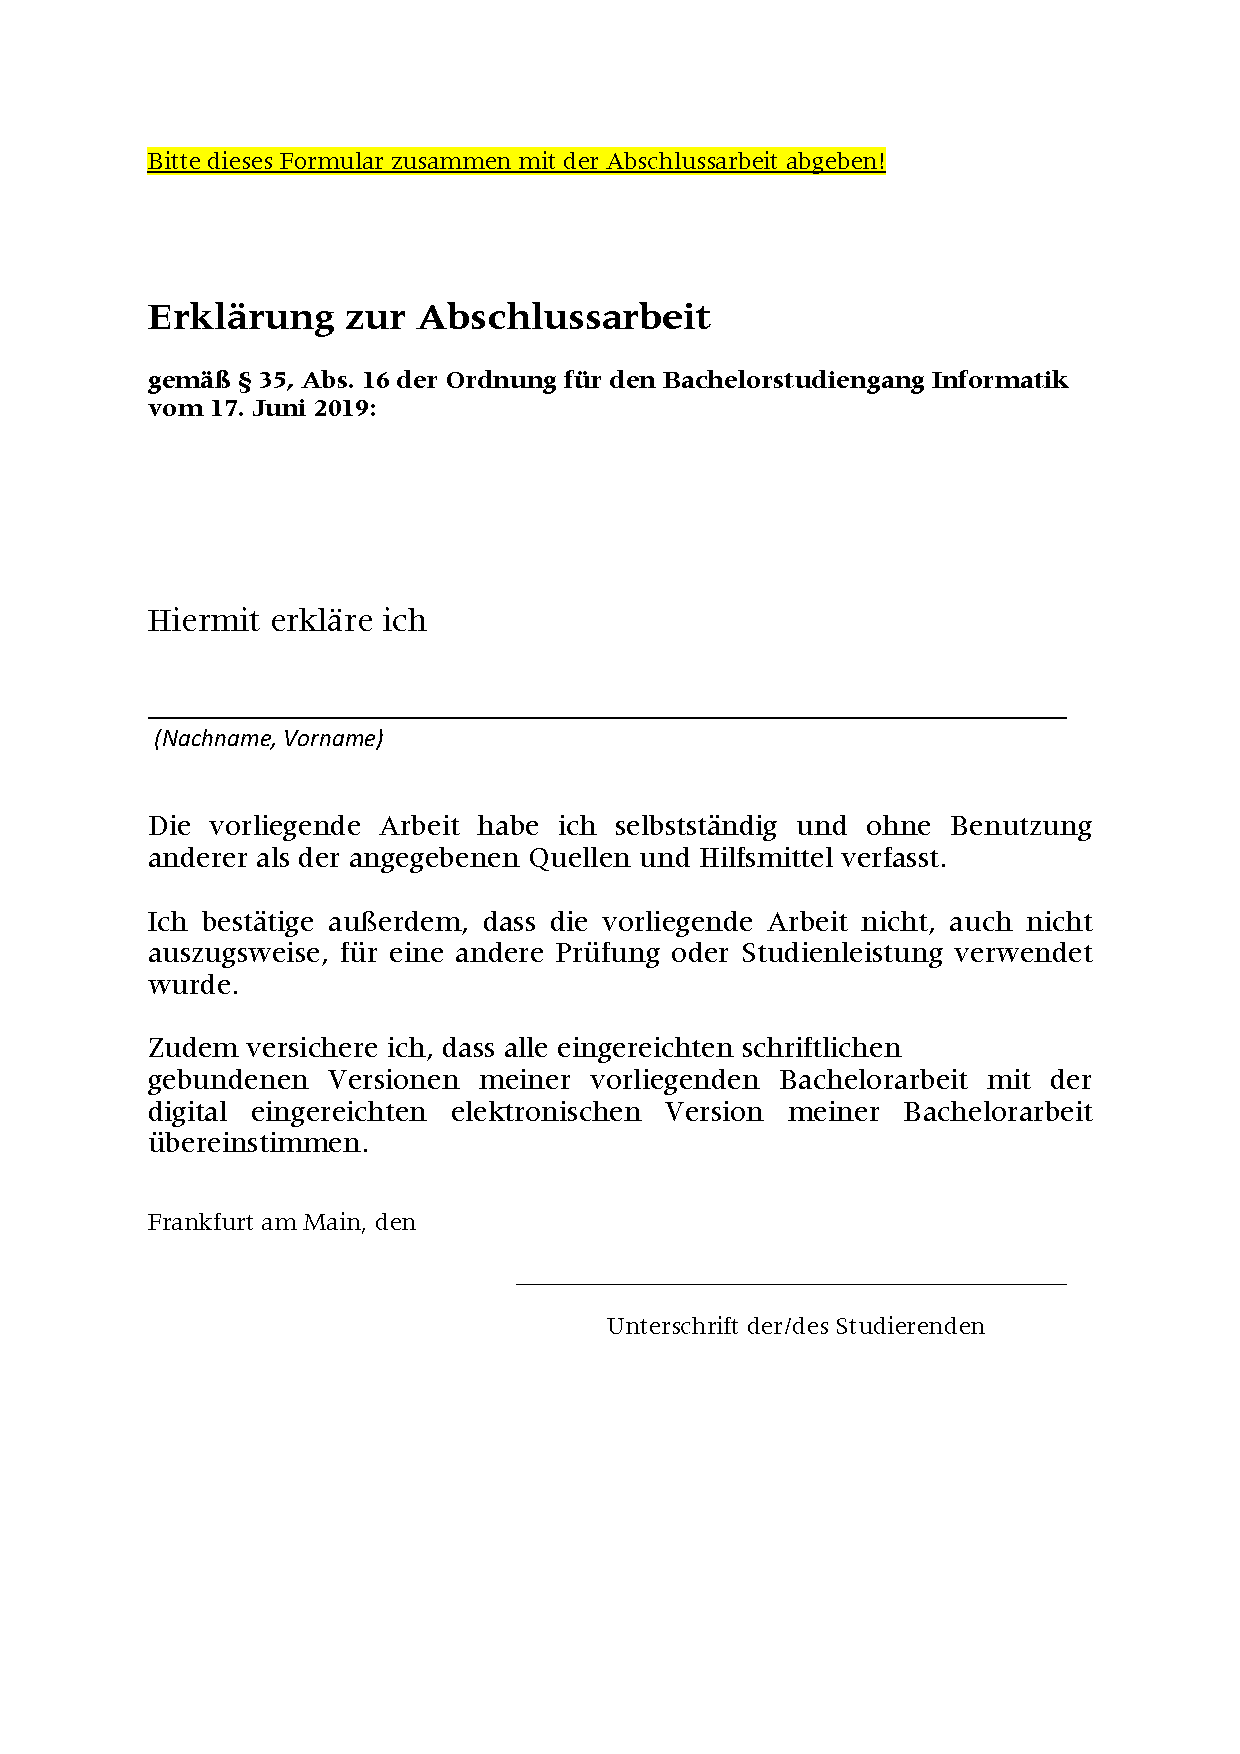
\includepdf[pages={1}]{04-back-matter/Erklaerung-Lisa.pdf}
	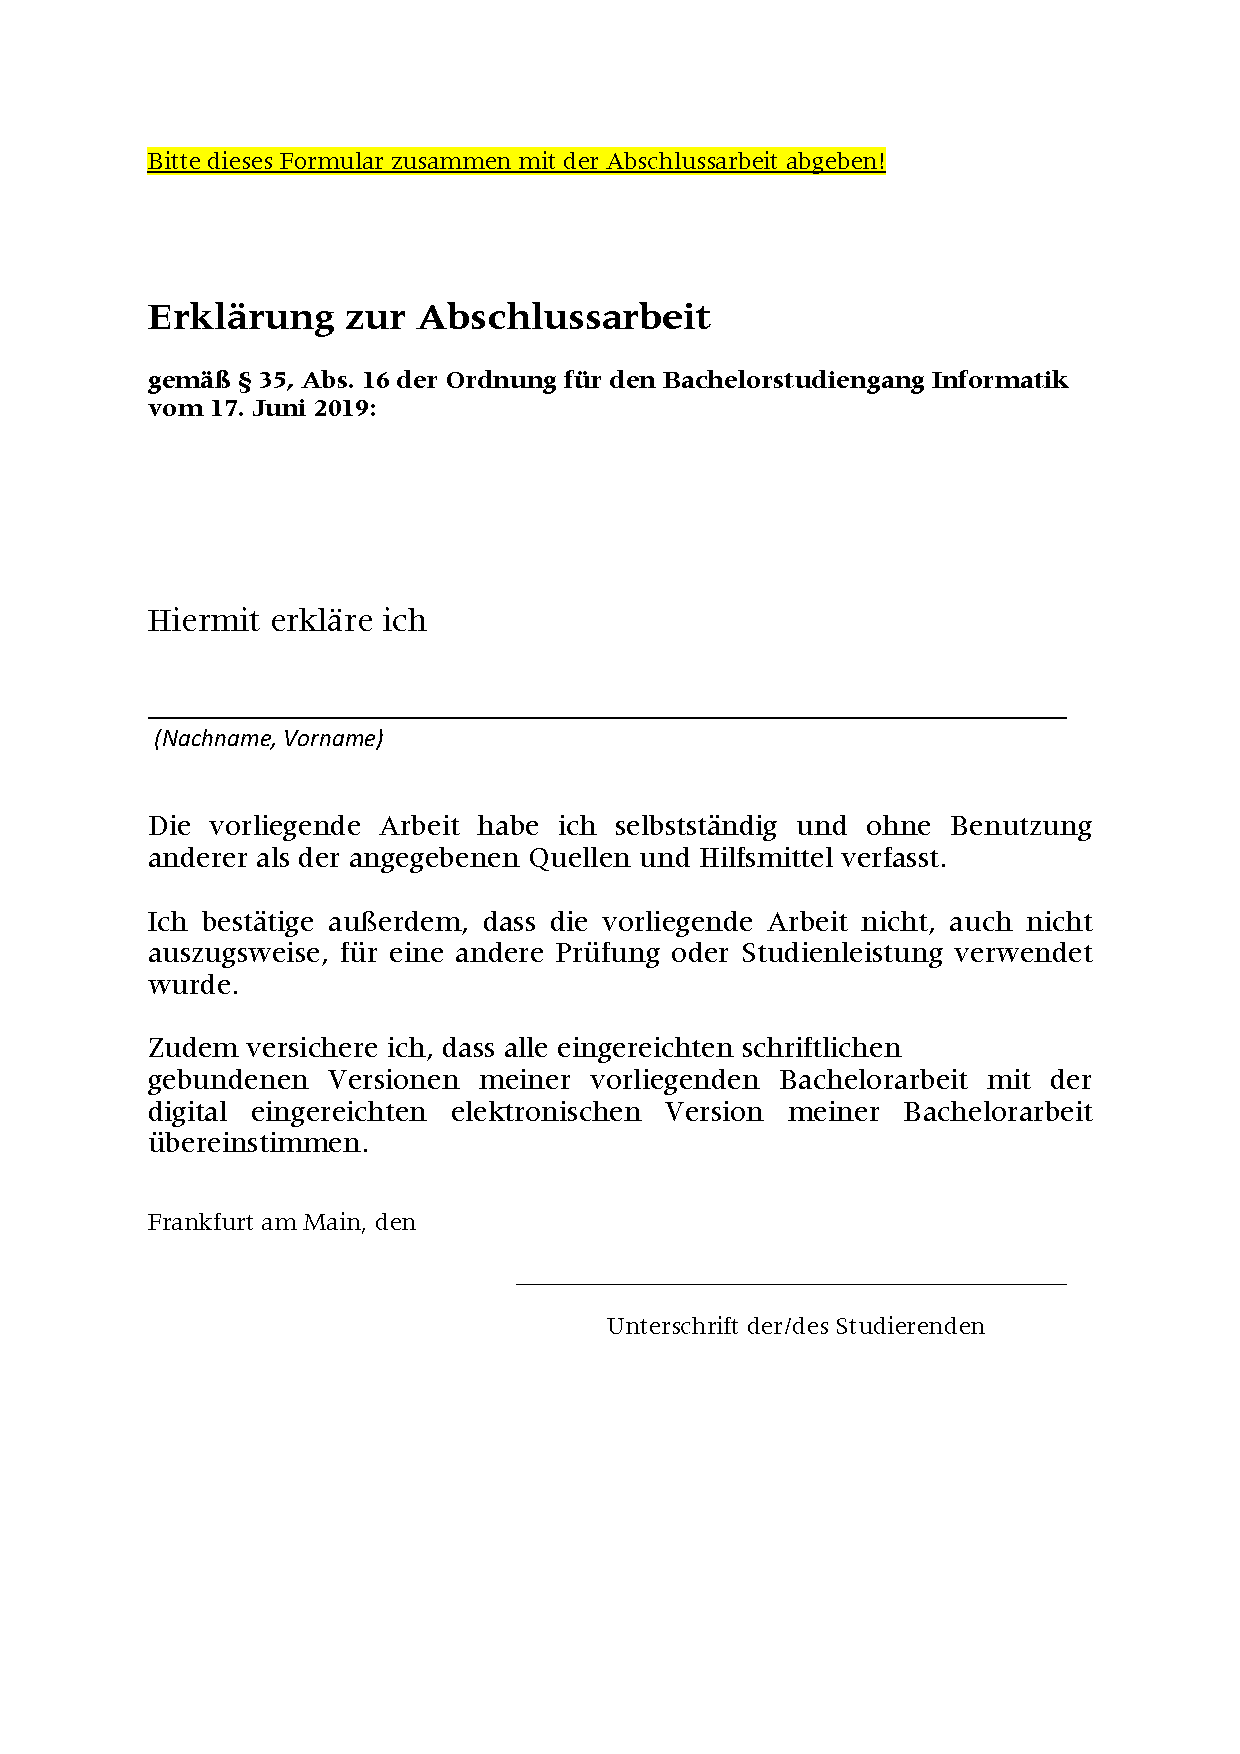
\includepdf[pages={1}]{04-back-matter/Erklaerung-Domi.pdf}
}

%********************************************************************
% Game Over: Restore, Restart, or Quit?
%*******************************************************
\end{document}
%********************************************************************
